\documentclass[11pt]{article}

\usepackage[margin=1in]{geometry}
\usepackage{fontspec}
\usepackage{microtype}
\usepackage{amsmath,amssymb,amsthm}
\usepackage{mathtools}
\usepackage{xcolor}
\usepackage{hyperref}
\usepackage{booktabs}
\usepackage{enumitem}
\usepackage{listings}
\usepackage{tikz}
\usetikzlibrary{arrows.meta,positioning,shapes.geometric,calc,fit,decorations.pathreplacing}

\hypersetup{
  colorlinks=true,
  linkcolor=blue!50!black,
  citecolor=blue!50!black,
  urlcolor=blue!50!black
}

\setmainfont{Latin Modern Roman}
\setsansfont{Latin Modern Sans}
\setmonofont{DejaVu Sans Mono}[Scale=MatchLowercase]

\lstdefinelanguage{Lean4}{
  morekeywords={
    import,namespace,end,open,section,noncomputable,abbrev,structure,inductive,
    def,theorem,lemma,where,match,with,if,then,else,by,fun,let,in,return,do,
    simp,calc,have,show,exact,rcases,cases,constructor,intro,apply,
    deriving,instance,class,extends,private,protected,mutual,partial,
    Type,Prop,Sort,Nat,Bool,true,false,sorry,axiom
  },
  sensitive=true,
  morecomment=[l]{--},
  morecomment=[s]{/-}{-/},
  morestring=[b]"
}

\lstset{
  language=Lean4,
  basicstyle=\ttfamily\small,
  keywordstyle=\bfseries\color{blue!50!black},
  commentstyle=\itshape\color{green!40!black},
  stringstyle=\color{red!50!black},
  showstringspaces=false,
  breaklines=true,
  frame=single,
  framerule=0.3pt,
  xleftmargin=0.5em,
  xrightmargin=0.5em,
  keepspaces=true,
  columns=fullflexible
}

\newtheorem{theorem}{Theorem}[section]
\newtheorem{lemma}[theorem]{Lemma}
\newtheorem{definition}[theorem]{Definition}
\newtheorem{fact}[theorem]{Fact}
\theoremstyle{remark}
\newtheorem{remark}[theorem]{Remark}

\newcommand{\MeTTa}{\textup{MeTTa}}
\newcommand{\MeTTaIL}{\textup{MeTTaIL}}
\newcommand{\MORK}{\textup{MORK}}
\newcommand{\PathMap}{\textup{PathMap}}
\newcommand{\PeTTa}{\textup{PeTTa}}
\newcommand{\HE}{\textup{HE}}
\newcommand{\code}[1]{\texttt{#1}}
\newcommand{\codepath}[1]{\path{#1}}
\newcommand{\leanref}[1]{\texttt{#1}}
\newcommand{\TODO}[1]{\textcolor{red!60!black}{[TODO: #1]}}

% TikZ styles
\tikzset{
  archbox/.style={draw, rounded corners=3pt, minimum width=2.8cm,
    minimum height=0.7cm, align=center, font=\small\sffamily},
  proofbox/.style={archbox, fill=blue!8, draw=blue!40!black},
  rtbox/.style={archbox, fill=orange!8, draw=orange!50!black},
  sharedbox/.style={archbox, fill=green!8, draw=green!40!black},
  neutralbox/.style={archbox, fill=gray!8, draw=gray!50!black},
  arrw/.style={-{Stealth[length=5pt]}, thick},
  darrw/.style={-{Stealth[length=5pt]}, thick, dashed},
}

\title{PureMeTTa\\
\large Architecture for \MeTTa-Pure, Elaborated \MeTTa-Core,\\
Runtime Execution, and Overlap Certificates}
\author{Zar \and Oru\v{z}i\footnote{``Oru\v{z}i'' denotes AI-assisted
collaboration using Claude Code (Anthropic), ChatGPT, and Codex (OpenAI).}}
\date{March 2026}

\begin{document}
\maketitle

\begin{abstract}
This document records the current \MeTTa{} architecture as formalized in Lean~4.
The central claim is that the project should converge to a single elaborated
\MeTTa-Core that compiles to two honest targets: a trusted proof-oriented kernel
(\MeTTa-Pure / PureKernel) and an efficient runtime execution seam
(\MORK{}/MM2-backed \code{RuntimeExec}).

The document is anchored in the code: every key claim cites the Lean file and
theorem name where it is proved. The current proof-side center is no longer
just an abstract certificate interface: it is a small closed-fragment semantic
waist with canonical normalization by complete development, bidirectional
checking, and parser-free checked canonical evaluation with preservation.

We describe the current proven overlap (artifact-only for Pure, direct execution
for \PeTTa{}/MM2-backed fragments), the runtime kernel classes
(exec + query + space effect + oracle + meta), the restricted Pure certificate
lane, the current ordinary-family spec/interface stack, and the concrete next
steps toward a genuinely dual-target fragment.
\end{abstract}

\tableofcontents

%% ====================================================================
\section{Thesis}
\label{sec:thesis}

The working thesis is:

\begin{quote}
One surface \MeTTa{} should elaborate to one shared \MeTTa-Core, which then
lowers to two distinct but connected targets:
\begin{enumerate}[nosep]
  \item a proof-oriented target: \MeTTa-Pure / PureKernel;
  \item a runtime target: \MeTTaIL{} artifacts / \code{RuntimeExec} /
  \MORK{}/MM2 / Rust execution.
\end{enumerate}
\end{quote}

This is intended to be closer to the Lean-style pattern

\begin{center}
\fbox{\parbox{0.88\linewidth}{
surface language $\to$ elaborated core $\to$ checked kernel and compiled runtime
}}
\end{center}

than to either of the following extremes:

\begin{enumerate}[nosep]
  \item runtime \emph{is} the proof kernel;
  \item proof language and runtime language stay permanently separate and only
  meet in a semantic backstop such as world-model consequence.
\end{enumerate}

%% ====================================================================
\section{Current Architecture}
\label{sec:arch}

\subsection{System Diagram}

\begin{center}
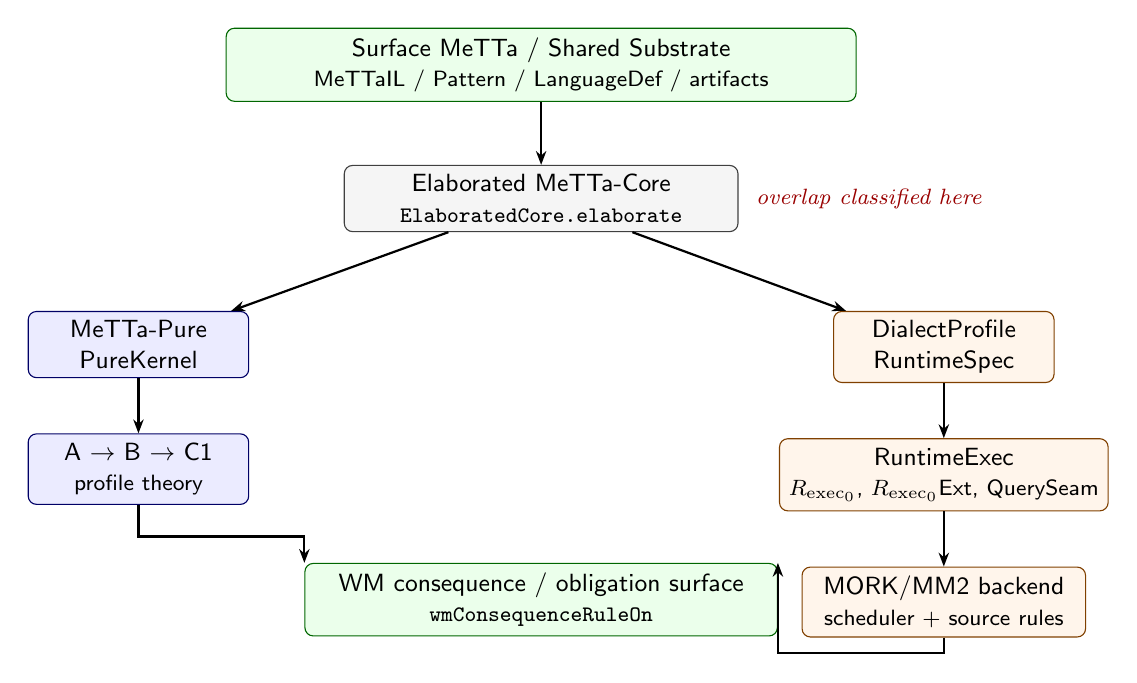
\begin{tikzpicture}[node distance=1.1cm and 1.8cm]
  % Surface
  \node[sharedbox, minimum width=8cm] (surface)
    {Surface \MeTTa{} / Shared Substrate\\
     \footnotesize\MeTTaIL{} / Pattern / LanguageDef / artifacts};

  % Elaborated Core
  \node[neutralbox, minimum width=5cm, below=0.8cm of surface] (elab)
    {Elaborated \MeTTa-Core\\
     \footnotesize\leanref{ElaboratedCore.elaborate}};

  % Proof branch
  \node[proofbox, below left=1.0cm and 1.2cm of elab] (pure)
    {\MeTTa-Pure\\PureKernel};
  \node[proofbox, below=0.7cm of pure] (abc)
    {A $\to$ B $\to$ C1\\
     \footnotesize profile theory};

  % Runtime branch
  \node[rtbox, below right=1.0cm and 1.2cm of elab] (rtspec)
    {DialectProfile\\RuntimeSpec};
  \node[rtbox, below=0.7cm of rtspec] (rtexec)
    {RuntimeExec\\
     \footnotesize $R_{\mathrm{exec}_0}$, $R_{\mathrm{exec}_0}$Ext, QuerySeam};
  \node[rtbox, below=0.7cm of rtexec, minimum width=3.6cm] (mork)
    {\MORK{}/MM2 backend\\
     \footnotesize scheduler $+$ source rules};

  % WM surface
  \node[sharedbox, minimum width=6cm,
        below=4.2cm of elab] (wm)
    {WM consequence / obligation surface\\
     \footnotesize\leanref{wmConsequenceRuleOn}};

  % Arrows
  \draw[arrw] (surface) -- (elab);
  \draw[arrw] (elab) -- (pure);
  \draw[arrw] (elab) -- (rtspec);
  \draw[arrw] (pure)  -- (abc);
  \draw[arrw] (rtspec) -- (rtexec);
  \draw[arrw] (rtexec) -- (mork);
  \draw[arrw] (abc.south) -- ++(0,-0.4) -| (wm.north west);
  \draw[arrw] (mork.south) -- ++(0,-0.2) -| (wm.north east);

  % Overlap annotation
  \node[font=\footnotesize\itshape, text=red!60!black,
        right=0.1cm of elab.east, anchor=west] {overlap classified here};
\end{tikzpicture}
\end{center}

\medskip
\noindent
The important present facts are:

\begin{enumerate}
  \item \MeTTa-Pure and PureKernel are real and theorem-level strong, and the
  current closed proof-side waist is now packaged as a checking /
  normalization / evaluation service.
  \item \code{RuntimeExec} is real and theorem-level strong over the current
  \MORK{}/MM2 seam.
  \item The current strongest shared semantic meeting point is the WM
  consequence / obligation surface.
  \item The elaborated core classifies overlap honestly:\\
  \leanref{OverlapClass.artifactOnly} vs.\
  \leanref{OverlapClass.directExec}.
  \item This is honest, but not yet the desired end state.
\end{enumerate}

\subsection{The Proof Branch}
\label{sec:proof-branch}

The current proof branch is:

\begin{center}
\MeTTa-Pure $\;\to\;$ PureKernel $\;\to\;$ A $\;\to\;$ B $\;\to\;$ C1
\end{center}

\noindent
where:

\begin{itemize}
  \item \textbf{A} is the tiny closed executable kernel fragment
  (operational steps via \leanref{pureOpStep});
  \item \textbf{B} is kernel theory reduction
  (profile theory via \leanref{PureKernel.ProfileTheory});
  \item \textbf{C1} is the quoted profile-theory closure
  (\leanref{quoteClosed\-Tm} bridge).
\end{itemize}

\paragraph{Key theorems.}
\begin{itemize}
  \item \leanref{pureClosedTheoryBridge\_to\_star} --- one-step bridge lifts
  to reflexive-transitive closure by induction.
  \item \leanref{profileStepStar\_sound} --- star closure transports to WM
  inequalities.
  \item \leanref{pureTheoryStep\_to\_wmStrengthObligation\_default} ---
  PureKernel reduction $\to$ WM obligation via the canonical bridge.
\end{itemize}

\paragraph{Primary files.}
\begin{itemize}
  \item \codepath{Mettapedia/Languages/MeTTa/Pure/Core.lean}
  --- \leanref{PureTm}, \leanref{mettaPure} dialect definition.
  \item \codepath{Mettapedia/Languages/MeTTa/PureKernel/CoreEmbedding.lean}
  --- kernel embedding, profile theory.
  \item \codepath{Mettapedia/Languages/MeTTa/PureKernel/PatternBridge.lean}
  --- quotation, \leanref{quoteClosedTm}.
  \item \codepath{Mettapedia/Logic/PLNWorldModelPureKernelBridge.lean}
  --- \leanref{PureJudgmentWMInterface}, WM landing.
\end{itemize}

\noindent
This branch is not aspirational. It is already theorem-level packaged with
0~sorry.

\subsection{The Current Closed Semantic Waist}
\label{sec:semantic-waist}

The current proof-side reference model should not be identified with the
CLI-level fuel evaluator alone. The authoritative center is the closed Pure
semantic waist exposed above \leanref{PureCheckingBoundary}.

\paragraph{Canonical normalization and definitional equality.}
\codepath{Mettapedia/Languages/MeTTa/PureNormalizationService.lean}
packages the current closed reference normalization service around complete
development \leanref{cdev}. The central object is
\leanref{CanonicalClosedPureTerm}, constructed by
\leanref{canonicalizeClosedPureTerm}. It carries:
\begin{itemize}[nosep]
  \item the input closed term,
  \item its canonical development,
  \item a \leanref{RedStar} reduction to that canonical development,
  \item a conversion proof \leanref{Conv} to that canonical development.
\end{itemize}

\noindent
The same module also exposes the current closed service operations:
\begin{itemize}[nosep]
  \item \leanref{defEqClosed?},
  \item \leanref{asPiClosed?},
  \item \leanref{asSigmaClosed?},
  \item boundary wrappers such as
  \leanref{PureCheckingBoundary.canonicalizeClosed}.
\end{itemize}

\paragraph{Bidirectional checking.}
\codepath{Mettapedia/Languages/MeTTa/PureBidirectionalChecking.lean}
packages closed surface checking through \leanref{PureCheckSuccess},
\leanref{inferSurfacePure}, and \leanref{checkSurfacePure}. Parser-free checked
canonical evaluation then lives in
\codepath{Mettapedia/Languages/MeTTa/PureCanonicalEvaluation.lean}:
\begin{itemize}[nosep]
  \item \leanref{CheckedCanonicalEvaluation},
  \item \leanref{PureCheckingBoundary.checkAndCanonicalizeClosedTerm},
  \item \leanref{PureCheckingBoundary.checkAndEvalSurface},
  \item \leanref{subjectReductionRedStar}.
\end{itemize}

\paragraph{Executable/canonical agreement.}
The executable stepper remains important, but now in the right role. In
\paragraph{Current service view.}
The current live Pure-facing proof services now land on the same semantic
waist, but the live entry points are theoremic services rather than the
archived prototype CLI tools:

\begin{center}
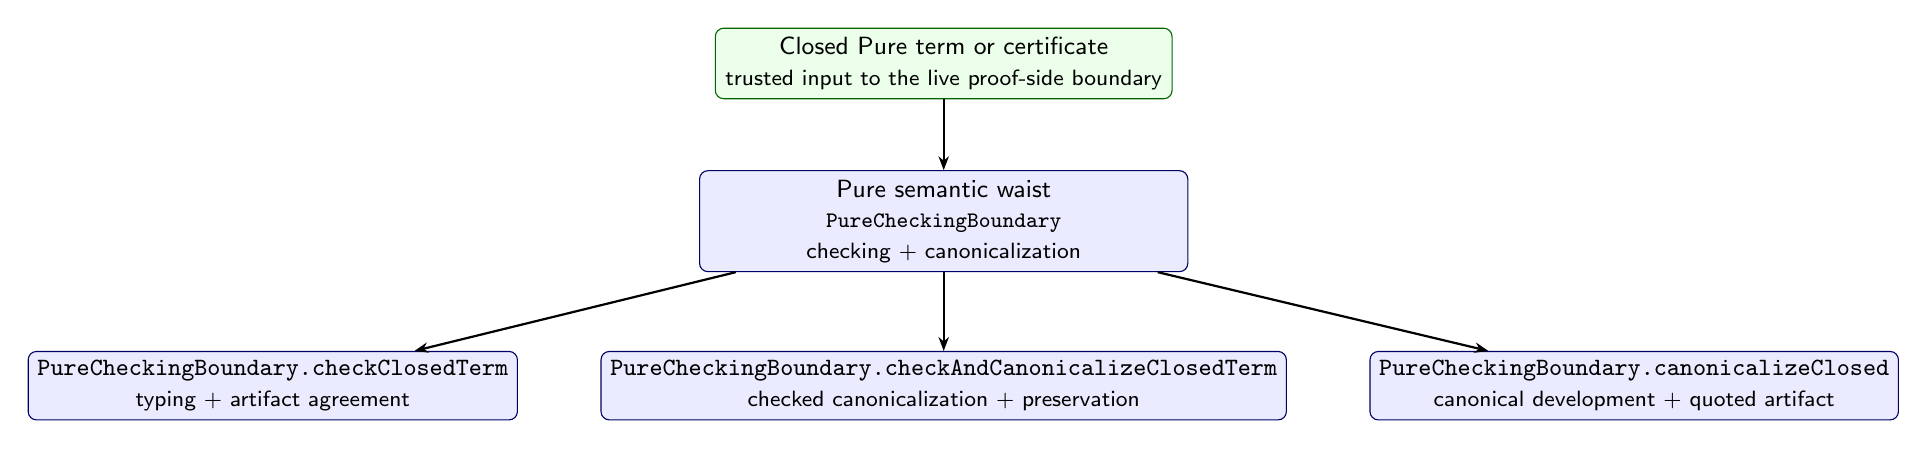
\begin{tikzpicture}[node distance=0.9cm and 1.2cm]
  \node[sharedbox, minimum width=5.8cm] (surface)
    {Closed Pure term or certificate\\
     \footnotesize trusted input to the live proof-side boundary};

  \node[proofbox, below=0.9cm of surface, minimum width=6.2cm] (waist)
    {Pure semantic waist\\
     \footnotesize \leanref{PureCheckingBoundary}\\
     \footnotesize checking + canonicalization};

  \node[proofbox, below left=1.0cm and 2.3cm of waist, minimum width=3.6cm] (check)
    {\leanref{PureCheckingBoundary.checkClosedTerm}\\
     \footnotesize typing + artifact agreement};

  \node[proofbox, below=1.0cm of waist, minimum width=3.8cm] (checkeval)
    {\leanref{PureCheckingBoundary.checkAndCanonicalizeClosedTerm}\\
     \footnotesize checked canonicalization + preservation};

  \node[proofbox, below right=1.0cm and 2.3cm of waist, minimum width=3.9cm] (agree)
    {\leanref{PureCheckingBoundary.canonicalizeClosed}\\
     \footnotesize canonical development + quoted artifact};

  \draw[arrw] (surface) -- (waist);
  \draw[arrw] (waist) -- (check);
  \draw[arrw] (waist) -- (checkeval);
  \draw[arrw] (waist) -- (agree);
\end{tikzpicture}
\end{center}

\noindent
This is now a deliberately parser-free proof-side service arrangement rather
than a front-door evaluator. The archived prototype CLI was useful for
exploration, but the live trusted path is the theoremic checking and
canonicalization boundary itself.

\paragraph{Worked example.}
Consider the tiny closed Pure program represented directly as the closed kernel
term \leanref{PureTm.app} of the identity lambda applied to \leanref{PureTm.u0}.
The corresponding type judgment is the closed theorem that the input has type
\code{Type1}.

\begin{lstlisting}
input            := ((lambda x. x) Type0)
claimedType      := Type1
inputTyping      : HasType nil input claimedType
\end{lstlisting}

\noindent
Applying
\leanref{PureCheckingBoundary.checkAndCanonicalizeClosedTerm} to this input
currently yields a theoremic record of the following shape:

\begin{lstlisting}
input: ((lambda x. x) Type0)
claimedType: Type1
canonical-development: (Type0)
input-artifact: Pattern.apply "App" [...]
canonical-artifact: Pattern.apply "U0" []
proof: inputTyping : HasType nil input Type1
proof: outputTyping : HasType nil canonicalDevelopment Type1
proof: canonical-quoted-artifact-agreement
proof: profile-bridge
\end{lstlisting}

\noindent
The key educational point is that \code{Type1} here is the \emph{type of the
input term}, not the evaluation result. The term evaluates to \code{Type0}, and
the reason the check succeeds is that the current Pure kernel proves
\code{Type0 : Type1}.

\medskip
\noindent
So even this tiny example already exhibits the live waist:
closed checking, canonicalization by complete development, quotation into the
shared artifact substrate, and profile-theory transport from the canonical
reduction.

\paragraph{Why this already matters.}
This is enough to prevent the current Pure waist from being ``only esoteric
theory.'' The present closed fragment already supports:
\begin{itemize}[nosep]
  \item trusted checking into \leanref{PureTm},
  \item canonical normalization and definitional equality,
  \item parser-free checked canonical evaluation with preservation,
  \item quotation into the shared \MeTTaIL{} artifact space.
\end{itemize}

\noindent
What this \emph{does not} yet mean is direct MM2/\MORK{} operational overlap.
The current sense in which it is already a strain of \MeTTa{} is that the
surface syntax, artifact substrate, and elaborated-core story are shared, while
the proof-side operational account remains an honest closed-fragment kernel
waist.

\subsection{What ``Kernel Binders'' Means Here}
\label{sec:kernel-binders}

The phrase ``kernel binders'' is doing important work in this paper. In the
current Pure fragment, the binding forms belong to the trusted internal term
language itself:
\begin{itemize}[nosep]
  \item $\Pi$ for dependent function types,
  \item $\Sigma$ for dependent pair types,
  \item \leanref{lam} for lambda abstraction.
\end{itemize}

\noindent
These are not runtime closures or ad hoc higher-order macros. They are
constructors of \leanref{PureTm} with typing, reduction, substitution, and
conversion rules in the kernel theory. The preferred surface syntax
\code{(lambda \$x body)} is therefore a user-facing presentation of a real
kernel binder, not a disguised \code{apply}/\code{let} encoding.

\noindent
This distinction matters when comparing Pure against existing \MeTTa{}
practice:
\begin{itemize}[nosep]
  \item \textbf{Pure kernel binders} are part of the trusted proof-side syntax
  and can participate in checked typing, canonical normalization, and subject
  reduction.
  \item \textbf{Runtime closure forms} such as \PeTTa{}'s \code{|->} are
  operationally real and useful, but they are not currently the semantic center
  of the proof kernel.
  \item \textbf{Encoded ``lambda'' tricks} in some \HE{}/older \MeTTa{} usage
  are even further away: they may be practical higher-order surface devices,
  but they are not the same thing as kernel-level binders with theoremic
  typing and conversion.
\end{itemize}

\noindent
So when this paper says that Pure is already a real strain of \MeTTa{}, it does
not mean ``Pure already subsumes \PeTTa{} operationally.'' It means that Pure
already contributes a real typed binder language, expressed in \MeTTa{}-shaped
surface syntax, that lands in a trusted kernel and shared artifact substrate.

\subsection{The Runtime Branch}
\label{sec:runtime-branch}

The runtime branch passes through three layers:

\begin{center}
DialectProfile / RuntimeSpec $\;\to\;$ RuntimeExec $\;\to\;$ \MORK{}/MM2 seam
\end{center}

\paragraph{Three runtime surfaces.}
The central type is \leanref{MeTTaRuntimeExecSurface}
(\codepath{RuntimeExec.lean}), a structure with 8~fields including an
\emph{embedded proof}:

\begin{itemize}[nosep]
  \item \leanref{noPremiseBridge : RuntimeExecNoPremiseSourceBridge} ---
  proves that if a rule has \code{fvar}-headed LHS, translatable RHS, and
  no premises, then its template sinks fire correctly at the
  \MORK{} source-rule level.
\end{itemize}

Three canonical instances are constructed:

\begin{center}
\begin{tabular}{@{}llp{5.5cm}@{}}
\toprule
Instance & Name & Capability \\
\midrule
$R_{\mathrm{exec}_0}$ & \leanref{morkRuntimeExec0} &
  No-premise source-rule bridge \\
$R_{\mathrm{exec}_0}$Ext & \leanref{morkRuntimeExec0Ext} &
  Multi-premise + guarded bridge \\
QuerySeam & \leanref{morkRuntimeQueryExec0} &
  Query surface with \emph{soundness + completeness} proofs \\
\bottomrule
\end{tabular}
\end{center}

\paragraph{Query surface detail.}
\leanref{MeTTaRuntimeQuerySurface}
carries bidirectional correctness:
\begin{itemize}[nosep]
  \item \leanref{sourceFactorSound} --- computable results inject into
  spec-level results;
  \item \leanref{sourceFactorComplete} --- spec-level results extract from
  computable results.
\end{itemize}

\paragraph{Primary files.}
\begin{itemize}
  \item \codepath{Mettapedia/Languages/MeTTa/RuntimeExec.lean} (269~lines)
  --- surfaces, instances.
  \item \codepath{Mettapedia/Languages/ProcessCalculi/MORK/ExecutionBoundary.lean}
  (509~lines) --- 160+ re-exported theorems including
  \leanref{fireCorrespondence}, \leanref{schedulerProgress}.
  \item \codepath{Mettapedia/Languages/ProcessCalculi/MORK/DirectExecSurface.lean}
  (326~lines) --- composition package:
  \leanref{pettaEvalStep\_schedulerFires},
  \leanref{addAtomCmd\_schedulerFires}.
\end{itemize}

\subsection{Current Overlap Fact}
\label{sec:overlap-fact}

The current honest overlap is \emph{artifact-only}, not direct runtime
execution.

\begin{fact}[Pure/runtime frontier]
\label{fact:frontier}
No \code{mettaPure} rewrite rule currently fits the direct $R_{\mathrm{exec}_0}$
source-rule bridge.

\medskip\noindent
\textup{Lean:}
\leanref{no\_mettaPure\_rewrite\_fits\_direct\_runtimeExec0\_source\_bridge}
\textup{in} \codepath{PureRuntimeFrontier.lean}.
\end{fact}

\noindent
The real current overlap path is:

\begin{center}
closed Pure surface terms $\;\to\;$ PureKernel term $\;\to\;$
quoted / shared artifact
\end{center}

\noindent
proved by:
\begin{itemize}[nosep]
  \item \leanref{closedPure\_overlap\_via\_abc} --- artifact-only overlap
  via quotation.
  \item \leanref{closedPure\_overlap\_via\_abc\_to\_wm} --- extends to WM
  consequence.
  \item \leanref{surfacePureClosed\_overlap\_is\_not\_directExec}
  (\codepath{PureCertificateFragment.lean}).
  \item \leanref{surfaceCoreTypedAtom\_overlap\_is\_not\_directExec}
  (\codepath{ElaboratedCore.lean}).
\end{itemize}

\noindent
The current live proof-side services sharpen this further. Canonicalization by
\leanref{cdev} is exposed through
\leanref{PureCheckingBoundary.canonicalizeClosed}, and checked canonical
evaluation is exposed through
\leanref{PureCheckingBoundary.checkAndCanonicalizeClosedTerm}. This is
\emph{not} the same as a theorem that Pure evaluation is already direct
\MORK{}/MM2 execution. The current honest statement remains:
\begin{quote}
Pure closed terms have a real canonicalization service and a real
shared-artifact overlap witness, but they do not yet have direct
proof/runtime operational overlap.
\end{quote}

%% ====================================================================
\section{Why the Current Fork Is Not Enough}
\label{sec:why-fork}

The current fork is a good bootstrap, but not the desired final user story.

\begin{itemize}
  \item Positive: it prevents us from lying about overlap.
  \item Negative: it makes the system feel too much like ``proof \MeTTa{}''
  versus ``runtime \MeTTa{}''.
\end{itemize}

The missing piece is a genuine:

\begin{center}
\fbox{\parbox{0.75\linewidth}{
Elaborated \MeTTa-Core
}}
\end{center}

\noindent
that is stronger than WM-only unification and earlier than backend execution.

%% ====================================================================
\section{Elaborated \MeTTa-Core}
\label{sec:elab}

\subsection{Base Infrastructure}

The file \codepath{ElaboratedCoreBase.lean} (62~lines) defines the
neutral vocabulary shared by proof and runtime views:

\begin{itemize}[nosep]
  \item \leanref{ElaboratedRegion} (inductive, 4~constructors):
  \code{pureKernelRegion}, \code{runtimeExecRegion}, \code{oracleRegion},
  \code{metaRegion}.
  \item \leanref{SharedArtifact} (structure):
  a \leanref{Pattern} from the \MeTTaIL{} syntax layer.
  \item \leanref{RuntimeLowering} (inductive, 3~constructors):
  \code{exec}, \code{query}, \code{auditOnly}.
  \item \leanref{OverlapClass} (inductive, 2~constructors):
  \code{artifactOnly} (current honest state),
  \code{directExec} (reserved for future).
\end{itemize}

\subsection{Current Proof-of-Concept Elaborator}

The file \codepath{ElaboratedCore.lean} (414~lines, 0~sorry)
contains the PoC classifier.

\paragraph{Surface language.}
\leanref{SurfaceNode} is an inductive with 11~constructors:

\begin{center}
\small
\begin{tabular}{@{}lll@{}}
\toprule
Constructor & Region & Certificate type \\
\midrule
\code{surfacePureClosed} & pureKernel & \leanref{PureCertificate} \\
\code{coreTypedAtom} & pureKernel & \leanref{CoreTypedCertificate} \\
\code{pettaCoreRule} & runtimeExec & \leanref{PeTTaCoreRuleRuntimeCertificate} \\
\code{pettaSpaceCoreQuery} & runtimeExec & \leanref{PeTTaSpaceCoreRuntimeCertificate} \\
\code{heRuntimeRule/Query} & runtimeExec & \leanref{RuntimeCertificate} \\
\code{pettaRuntimeRule/Query} & runtimeExec & \leanref{RuntimeCertificate} \\
\code{fullLegacyRuntime} & runtimeExec & \leanref{RuntimeCertificate} \\
\code{oracleCall} & oracle & \leanref{OracleCertificate} \\
\code{metaQuoted} & meta & \leanref{MetaCertificate} \\
\bottomrule
\end{tabular}
\end{center}

\paragraph{Elaborated output.}
\leanref{ElaboratedNode} (inductive, 7~constructors):
\code{pureNode}, \code{coreTypedNode}, \code{pettaCoreRuleNode},
\code{pettaSpaceCoreNode}, \code{runtimeNode}, \code{oracleNode},
\code{metaNode}.

\paragraph{Main elaborator.}
\leanref{elaborate : SurfaceNode $\to$ ElaboratedNode} maps all
11~surface types to their classified outputs.

\paragraph{Preservation theorems (all proved).}
\begin{itemize}[nosep]
  \item 7~region-preservation theorems (e.g.\
  \leanref{elaborate\_surfacePureClosed\_region}).
  \item 5~artifact-preservation theorems (e.g.\
  \leanref{elaborate\_surfacePureClosed\_artifact}).
  \item Backend agreement:
  \leanref{runtimeBackendAgreement} --- \HE{} and \PeTTa{} target the same
  \MORK{}/MM2 backend.
\end{itemize}

\subsection{What Should Change Next}

The elaborated core should gradually stop naming runtime fragments by witness
dialect and instead classify them by semantic role.

The likely neutral runtime-facing classes are:

\begin{enumerate}[nosep]
  \item \code{ruleExecNode} (match-rewrite)
  \item \code{queryNode} (read-only space query)
  \item \code{spaceEffectNode} (stateful mutation)
  \item \code{oracleNode} (external/grounded)
  \item \code{metaNode} (elaboration-time)
  \item \code{pureNode} (proof-side)
\end{enumerate}

\TODO{Refactor the current dialect-specific runtime constructors in
\code{SurfaceNode} to these neutral classes.}

%% ====================================================================
\section{Current Proven Overlap vs.\ Intended Overlap}
\label{sec:overlap}

This section states the overlap situation precisely.

\subsection{Pure Overlap: Artifact-Only}

The three \code{mettaPure} rewrite rules are classified exactly by
\leanref{mettaPure\_rewrites\_exact} (\code{rfl} proof):

\begin{center}
\small
\begin{tabular}{@{}llll@{}}
\toprule
Rule & LHS shape & RHS translatable? & Fits $R_{\mathrm{exec}_0}$? \\
\midrule
BetaPi & apply-headed & No (\code{.subst}) & No \\
BetaSigmaFst & apply-headed & Yes (atom-only) & No \\
BetaSigmaSnd & apply-headed & Yes (atom-only) & No \\
\bottomrule
\end{tabular}
\end{center}

\noindent
No rule has an \code{fvar}-headed LHS
(\leanref{mettaPure\_rewrite\_lhs\_not\_fvar}),
and BetaPi uses \code{.subst} which is not \leanref{morkTranslatable}
(\leanref{betaPi\_rhs\_not\_morkTranslatable}).
Therefore:

\begin{fact}[No direct Pure$\to$runtime bridge]
\leanref{no\_mettaPure\_rewrite\_fits\_direct\_runtimeExec0\_source\_bridge}:
no \code{mettaPure} rule satisfies both \code{fvar}-LHS and
\leanref{morkTranslatable}-RHS simultaneously.
\end{fact}

\noindent
Current Pure overlap goes through quotation:
\leanref{closedPure\_overlap\_via\_abc} $\to$
\leanref{closedPure\_overlap\_via\_abc\_to\_wm}.

\subsection{Runtime Overlap: Direct Execution for PeTTa/MM2 Fragments}

Direct runtime execution \emph{does} exist for the \PeTTa{}/MM2-backed
fragments:

\begin{itemize}[nosep]
  \item \leanref{evalStep\_toMorkSourceFire} --- core eval step lands on
  $R_{\mathrm{exec}_0}$ source-rule boundary.
  \item \leanref{evalcStep\_toMorkSourceFire} --- same for \code{evalc}.
  \item \leanref{pettaEvalStep\_schedulerFires} --- fires through the
  full MM2/\MORK{} scheduler seam (3-phase refinement).
\end{itemize}

\subsection{The Gap}

Direct proof/runtime overlap is \textbf{not yet proved}. No surface
fragment currently satisfies \emph{both} PureKernel reduction \emph{and}
$R_{\mathrm{exec}_0}$ source-rule bridge simultaneously.

\begin{center}
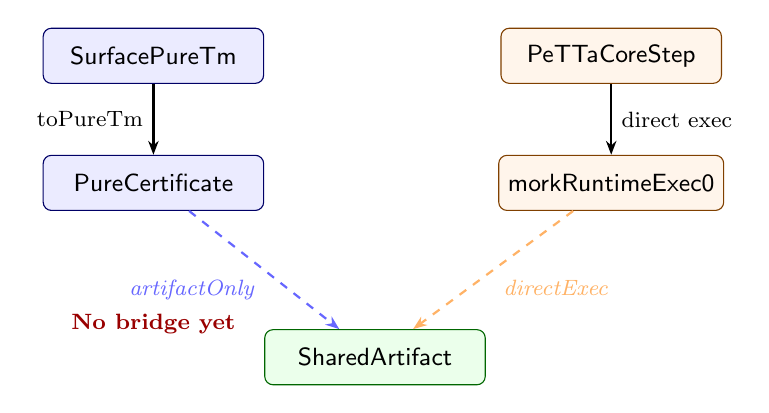
\begin{tikzpicture}[node distance=0.9cm and 2.5cm]
  \node[proofbox] (sptm) {SurfacePureTm};
  \node[proofbox, below=of sptm] (pcert) {PureCertificate};
  \node[rtbox, right=3cm of sptm] (pcs) {PeTTaCoreStep};
  \node[rtbox, below=of pcs] (rexec) {morkRuntimeExec0};

  \node[sharedbox, below right=1.5cm and 0cm of pcert] (sa) {SharedArtifact};

  \draw[arrw] (sptm) -- node[left,font=\footnotesize]{toPureTm} (pcert);
  \draw[arrw] (pcs) -- node[right,font=\footnotesize]{direct exec} (rexec);
  \draw[darrw, blue!60] (pcert) -- node[below left,font=\footnotesize\itshape]
    {artifactOnly} (sa);
  \draw[darrw, orange!60] (rexec) -- node[below right,font=\footnotesize\itshape]
    {directExec} (sa);

  \node[font=\footnotesize\bfseries\color{red!60!black},
        below=2.8cm of sptm, anchor=north] {No bridge yet};
\end{tikzpicture}
\end{center}

\subsection{Next Objective}

The next objective is a \emph{genuinely dual-target fragment}: a small
surface subset that elaborates to both a PureKernel certificate and a
direct $R_{\mathrm{exec}_0}$ source-rule firing, sharing the same artifact.
The likely candidate avoids \code{.subst} and uses symbolic atoms with
top-rule rewrite patterns.

%% ====================================================================
\section{Runtime Kernel Classes}
\label{sec:rt-kernel}

The runtime kernel should be understood not as ``just exec'' but as five
semantic classes over one default space model:

\begin{center}
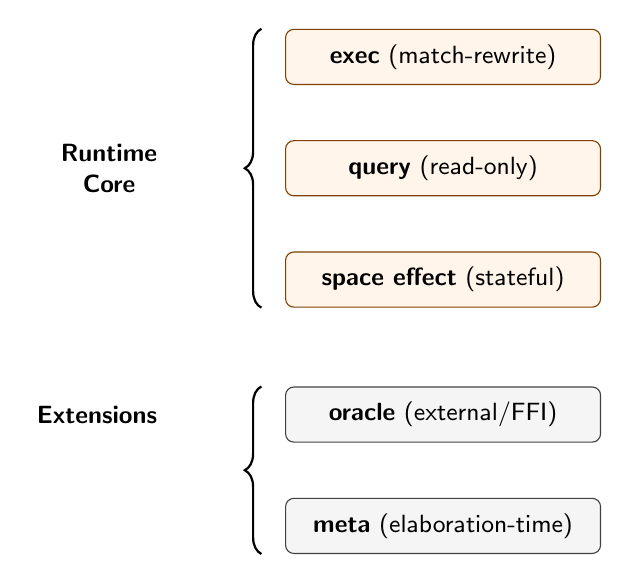
\begin{tikzpicture}[node distance=0.7cm and 1.5cm]
  \node[rtbox, minimum width=4cm] (exec)
    {\textbf{exec} (match-rewrite)};
  \node[rtbox, minimum width=4cm, below=of exec] (query)
    {\textbf{query} (read-only)};
  \node[rtbox, minimum width=4cm, below=of query] (effect)
    {\textbf{space effect} (stateful)};

  \node[neutralbox, minimum width=4cm, below=1cm of effect] (oracle)
    {\textbf{oracle} (external/FFI)};
  \node[neutralbox, minimum width=4cm, below=of oracle] (meta)
    {\textbf{meta} (elaboration-time)};

  \node[font=\small\sffamily\bfseries, align=center, left=1.5cm of query]
    (core) {Runtime\\Core};
  \node[font=\small\sffamily\bfseries, align=center, left=1.5cm of oracle]
    (ext) {Extensions};

  \draw[thick, decorate, decoration={brace, amplitude=6pt, mirror}]
    ([xshift=-0.3cm]exec.north west) -- ([xshift=-0.3cm]effect.south west);
  \draw[thick, decorate, decoration={brace, amplitude=6pt, mirror}]
    ([xshift=-0.3cm]oracle.north west) -- ([xshift=-0.3cm]meta.south west);
\end{tikzpicture}
\end{center}

\subsection{Exec (Match-Rewrite)}

The central runtime primitive is the scheduler/source rewrite seam
over one space. The \MORK{}/MM2 formalization covers:

\begin{enumerate}[nosep]
  \item find \code{exec} facts in the space
  (\leanref{execFactsOfSpace});
  \item pick one by scheduler order
  (\leanref{selectNextExec},
  \codepath{WorkQueueOrder.lean});
  \item match its pattern against the read copy
  (\leanref{readCopy});
  \item apply template sinks to the live space
  (\leanref{fireExecFact},
  \codepath{ThreePhaseRefinement.lean}).
\end{enumerate}

\paragraph{Key theorems.}
\begin{itemize}[nosep]
  \item \leanref{fireCorrespondence}
  (\codepath{ExecutionBoundary.lean}) ---
  \code{DeclReduces} $\to$ \code{fireRule}.
  \item \leanref{schedulerProgress} --- selected exec fact $\Rightarrow$
  step exists.
  \item \leanref{pettaEvalStep\_schedulerFires},
  \leanref{pettaEvalcStep\_schedulerFires}
  (\codepath{DirectExecSurface.lean}) ---
  \PeTTa{} steps fire through the full scheduler seam.
\end{itemize}

\subsection{Query}

Queries are sibling primitives, not a disguised special case of \code{exec}.
The currently formalized query seam includes:

\begin{itemize}[nosep]
  \item \code{(match \&self \$x tmpl)} ---
  \leanref{anyFactMatch\_toMorkSourceQuery},
  \leanref{anyFactMatch\_toComputableSourceQuery}
  (\codepath{SpaceCoreFragment.lean}).
  \item \code{(get-atoms \&self)} ---
  \leanref{getAtoms\_toComputableSourceQuery}.
\end{itemize}

\noindent
The query surface \leanref{morkRuntimeQueryExec0}
(\codepath{RuntimeExec.lean}) carries bidirectional correctness:
soundness and completeness of computable matching against the spec-level
semantics.

\subsection{Space Effect}

Space mutations are explicit, not proof-kernel rewrites:

\begin{itemize}[nosep]
  \item \code{(add-atom \&self X)} ---
  \leanref{addAtomSourceExecRule}:
  template \code{[.remove cmd, .add X, .add ()]}.
  \item \code{(remove-atom \&self X)} ---
  \leanref{removeAtomSourceExecRule}:
  template \code{[.remove cmd, .remove X, .add ()]}.
\end{itemize}

\paragraph{Proved at scheduler level.}
\leanref{addAtomCmd\_schedulerFires},
\leanref{removeAtomCmd\_schedulerFires}
(\codepath{DirectExecSurface.lean}) ---
commands fire through the full \MORK{}/MM2 scheduler.
Pattern matching round-trips via \leanref{matchAtom\_addAtomCmdAtom}
(\codepath{SpaceEffectFragment.lean}).

\subsection{Oracle}

Grounded/FFI/resource calls are treated as \emph{oracle} forms.
The elaborated core already provides:

\begin{itemize}[nosep]
  \item \leanref{OracleCertificate} (\codepath{ElaboratedCore.lean}) ---
  fields: \code{dialect}, \code{opName}, \code{resultDescriptor},
  \code{args}, \code{artifact}.
  \item Region: \code{oracleRegion}.
\end{itemize}

\noindent
Oracle calls are runtime-relevant and potentially effectful.
They should remain explicit and not be silently treated as proof-kernel
computation.

\TODO{Grow the oracle certificate lane toward explicit
pre/post-condition contracts.}

\subsection{Meta}

Meta forms are elaboration-time/proof-time forms:

\begin{itemize}[nosep]
  \item \leanref{MetaCertificate} (\codepath{ElaboratedCore.lean}) ---
  fields: \code{description}, \code{artifact}.
  \item Region: \code{metaRegion}.
\end{itemize}

\noindent
These should stay separated from ordinary runtime execution.

%% ====================================================================
\section{Restricted Pure Certificate Lane}
\label{sec:cert-lane}

The Pure certificate lane is the first real dual-view fragment:
a surface term maps to both a trusted PureKernel term and a shared
\MeTTaIL{} artifact, with proven agreement.

\subsection{Surface Language}

\leanref{SurfacePureTm}
(\codepath{PureCertificateFragment.lean}, 191~lines)
is an inductive parameterized by \code{n : Nat} (de~Bruijn depth)
with 12~constructors:

\begin{center}
\small
\begin{tabular}{@{}ll@{}}
\toprule
Constructor & Meaning \\
\midrule
\code{var (Fin n)} & de~Bruijn variable \\
\code{u0}, \code{u1} & universe levels \\
\code{pi}, \code{sigma} & $\Pi$-type, $\Sigma$-type (bind with $n{+}1$) \\
\code{id} & identity type \\
\code{lam} & $\lambda$-abstraction (bind with $n{+}1$) \\
\code{app}, \code{pair} & application, pairing \\
\code{fst}, \code{snd} & projections \\
\code{refl} & reflexivity proof \\
\bottomrule
\end{tabular}
\end{center}

\subsection{Embeddings}

Two maps out of \leanref{SurfacePureTm}:

\begin{enumerate}
  \item \leanref{toPureTm : SurfacePureTm\;n $\to$ PureTm\;n} ---
  structural embedding into the trusted kernel.
  \item \leanref{toClosedPattern : SurfacePureTm\;0 $\to$ Pattern} ---
  quotation into the shared \MeTTaIL{} artifact space.
\end{enumerate}

\begin{fact}[Quotation agreement]
\leanref{toClosedPattern\_eq\_quoteClosedTm}:
the surface quotation agrees with the kernel quotation for all closed terms.
Proved by structural induction over all 12~constructors
(\leanref{toPatternWith\_eq\_quoteTmWith}).
\end{fact}

\subsection{Certificates}

\begin{itemize}
  \item \leanref{PureCertificate} --- fields: \code{term} (closed
  \leanref{PureTm\;0}), \code{artifact}, \code{abcSurface}.
  \item \leanref{SharedPureOverlapCertificate} --- the first real
  dual-view object: surface term, trusted Pure term, shared artifact,
  all proved to agree.
  \item \leanref{certifySurfacePure} --- constructor that builds the
  overlap certificate from a surface term.
  \item \leanref{certifySurfacePure\_overlapClass} --- proves the
  result is \code{artifactOnly}.
\end{itemize}

\subsection{Current Scope and Limitations}

\begin{itemize}
  \item[\checkmark] Closed Pure terms (de~Bruijn index 0).
  \item[\checkmark] Closed type claims ($\Pi$, $\Sigma$, identity, universes).
  \item[\checkmark] Explicit proof-relevant certificate objects.
  \item[$\times$] No inductives yet.
  \item[$\times$] No broad Lean-proof import yet.
  \item[$\times$] No open terms (binder depth $> 0$).
\end{itemize}

\noindent
This is the right first certificate/checking target: small enough to be
auditable, rich enough to carry real type-theoretic content.

\subsection{Judgment-Typed Checked Imports}

The restricted lane is now stronger than a raw overlap wrapper. In
\codepath{PureCertificateFragment.lean} the current checked import object is:

\begin{itemize}[nosep]
  \item \leanref{CheckedPureCertificate} --- imported restricted certificate
  plus an explicit claimed closed type and an empty-context typing witness;
  \item \leanref{PureJudgmentKind} --- currently
  \code{closedTyping} and \code{quotedArtifactAgreement};
  \item \leanref{PureCertificateJudgment} --- a judgment-typed view over a
  checked imported certificate.
\end{itemize}

\noindent
The important theoremic point is that the proof lane now supports explicit
judgment forms, not only ad hoc overlap objects:

\begin{itemize}[nosep]
  \item \leanref{PureCertificateJudgment.closedTyping\_holds},
  \item \leanref{PureCertificateJudgment.quotedArtifactAgreement\_holds}.
\end{itemize}

\noindent
This is still intentionally narrow: it is a real restricted import/check lane,
but not broad Lean-proof import.

%% ====================================================================
\section{Ordinary Families: Current Declaration Checker}
\label{sec:inductives}

The kernel now contains the first real ordinary-family mechanism: a computable
declaration checker that validates and emits \leanref{DeclSpec}s for
ordinary strictly-positive inductive families, both non-parametric and
parametric.
This replaced a tower of interface scaffolding that had grown ahead of any
real kernel implementation.

\subsection{Declaration Environment and Signature Discipline}

Three files establish the authoritative declaration layer:

\begin{itemize}[nosep]
  \item \codepath{DeclarationEnv.lean} --- \leanref{DeclName},
  \leanref{DeclEntry}, \leanref{DeclEnv}, lookup helpers
  \leanref{typeOf?} and \leanref{valueOf?}.
  \item \codepath{DeclarationSpec.lean} --- \leanref{DeclSpec} (a closed name,
  type, and optional value), \leanref{envOfSpecs}, and the ordered signature
  discipline: \leanref{SignatureWellFormed}, \leanref{PrefixDeclSpecAdmissible}.
  \item \codepath{DeclarationSemantics.lean} --- typed and well-formed
  declaration environments, \leanref{HasTypeDecl}, \leanref{RedDecl},
  \leanref{DeclEnvWellFormed}.
\end{itemize}

\noindent
The signature discipline ensures declarations are added in a well-founded order:
every type and optional value in a spec may only refer to names already
in the prefix.

\subsection{Non-Parametric Checker}

\codepath{InductiveDecl.lean} (205~lines, 0~sorry) provides the first
Lean-\code{addInductive}-style checker for strictly-positive closed families:

\begin{itemize}[nosep]
  \item \leanref{CtorSpec} --- a constructor name and closed type
  \leanref{PureTm 0}.
  \item \leanref{IndDecl} --- a type name and list of \leanref{CtorSpec}s.
  \item Validation predicates: \leanref{notOccursConst},
  \leanref{occursOnlyPositively}, \leanref{strictlyPositive},
  \leanref{targetsFamily}, \leanref{namesDistinct} --- all computable
  \leanref{Bool}.
  \item \leanref{checkIndDecl} : \leanref{IndDecl} $\to$
  \leanref{Option (List DeclSpec)} --- validates names, targets, and strict
  positivity; emits the type spec (type $= U_0$) plus constructor specs.
\end{itemize}

\noindent
Standard instances and their checker certificates (all proved by
\code{decide}):
\begin{center}
\small
\begin{tabular}{@{}lll@{}}
\toprule
Value & Kind & Certificate \\
\midrule
\leanref{unitDecl} & \leanref{IndDecl} & \leanref{check\_unitDecl} \\
\leanref{boolDecl} & \leanref{IndDecl} & \leanref{check\_boolDecl} \\
\leanref{natDecl}  & \leanref{IndDecl} & \leanref{check\_natDecl} \\
\bottomrule
\end{tabular}
\end{center}

\noindent
Agreement with the hand-written pilot specs is also kernel-checked
(\leanref{unitDecl\_specs\_agree}, \leanref{boolDecl\_specs\_agree},
\leanref{natDecl\_specs\_agree}).

\noindent
Negative examples (all by \code{decide}): duplicate names, negative occurrence,
and wrong target each independently return \leanref{none}.

\subsection{Parametric Checker and Telescope Operations}

\codepath{Telescope.lean} (287~lines, 0~sorry) extends the checker to
parametric families.
The key insight is that \leanref{Ctx n} --- already the canonical dependent
context in \codepath{Context.lean} --- is the right telescope type; no new
inductive is needed.

\paragraph{Telescope operations.}
\begin{itemize}[nosep]
  \item \leanref{telescopePi} : \leanref{Ctx n} $\to$ \leanref{PureTm n} $\to$
  \leanref{PureTm 0} --- wrap a body in $\Pi$-binders from a context.
  \item \leanref{telescopeLam} : same shape, produces $\lambda$-abstractions.
\end{itemize}

\paragraph{Checker predicates (all \leanref{Bool}, polymorphic in depth).}
\begin{itemize}[nosep]
  \item \leanref{piArity} --- count leading $\Pi$-binders.
  \item \leanref{resultIsU0} --- after peeling $k$ binders, body is $U_0$.
  \item \leanref{matchingParamDomains} --- first $k$ $\Pi$-domains agree
  (by \code{BEq}).
  \item \leanref{isParamApp} --- term is \code{const}~$c$ applied to
  consecutive de~Bruijn variables.
  \item \leanref{targetsFamilyP} --- after peeling all $\Pi$'s, head is the
  family applied to the parameter variables.
\end{itemize}

\paragraph{Parametric inductive declaration.}
\leanref{ParamIndDecl} stores the type-former type as a closed term
(\leanref{typeFormerType : PureTm 0}) rather than a separate \code{numParams}
field; the parameter count is derived as
\leanref{piArity decl.typeFormerType}.
This subsumes non-parametric families
(\leanref{typeFormerType} $= U_0$ gives \code{numParams} $= 0$).

\paragraph{Checker.}
\leanref{checkParamIndDecl} : \leanref{ParamIndDecl} $\to$
\leanref{Option (List DeclSpec)} validates names, type-former result, parameter
domain agreement, target correctness, and strict positivity.
The first parametric example --- \code{List A} --- is verified by
\code{decide}:

\begin{center}
\small
\begin{tabular}{@{}ll@{}}
\toprule
Value & Certificate \\
\midrule
\leanref{listDecl}   & \leanref{check\_listDecl} \\
\leanref{unitDeclP}  & \leanref{check\_unitDeclP} \\
\leanref{boolDeclP}  & \leanref{check\_boolDeclP} \\
\leanref{natDeclP}   & \leanref{check\_natDeclP} \\
\bottomrule
\end{tabular}
\end{center}

\noindent
Backward compatibility: \leanref{liftToParam} embeds every \leanref{IndDecl}
into a \leanref{ParamIndDecl}, and the two checkers agree on the result
(proved by \code{decide} for Unit, Bool, Nat).

\subsection{Honest Status}

The term syntax (\codepath{Syntax.lean}) is still:
$\Pi$, $\Sigma$, Id, universes, $\lambda$, application, pairs, projections,
and reflexivity.
Declaration checking validates and emits \leanref{DeclSpec} entries; it does
\emph{not} add new term constructors for inductive types.
Runtime overlap for these family declarations remains \code{artifactOnly}.

\noindent
Deliberately deferred to later kernel layers:
\begin{itemize}[nosep]
  \item recursor generation,
  \item indexed families (Eq, Vec, Fin --- distinguishing uniform parameters
  from varying indices),
  \item induction-recursion,
  \item coinductives,
  \item structural fixpoints.
\end{itemize}

%% ====================================================================
\section{Why Legacy MeTTaFull Is Not the Primary Runtime Source}
\label{sec:legacy}

The \code{fullLegacyRuntime} constructor exists in \leanref{SurfaceNode}
(one of 11~constructors), but it is \emph{not} the primary runtime-core
witness.

\begin{enumerate}
  \item \textbf{It is a legacy spec-facing slice.}
  \leanref{RuntimeSpec} is deliberately dialect-facing and audit-facing:
  it records bindings, branching, context, native hooks, and collection control
  \emph{without} defining execution machinery.
  It does not carry embedded proofs the way \leanref{MeTTaRuntimeExecSurface}
  does.

  \item \textbf{Real execution witnesses are the \PeTTa{}/MM2-backed fragments.}
  The files with embedded proof-carrying structures are:
  \begin{itemize}[nosep]
    \item \codepath{PeTTa/CoreFragment.lean} ---
    \leanref{PeTTaCoreStep} (eval/evalc $\to$ \leanref{morkRuntimeExec0}).
    \item \codepath{PeTTa/SpaceCoreFragment.lean} ---
    \leanref{PeTTaSpaceCoreQuery} (match/get-atoms $\to$
    \leanref{morkRuntimeQueryExec0}).
    \item \codepath{PeTTa/SpaceEffectFragment.lean} ---
    add/remove $\to$ scheduler seam.
  \end{itemize}

  \item \textbf{MeTTaFull is not the best current witness for runtime-core
  development.}
  It packages the whole dialect profile without isolating the operational
  kernel. The current architecture deliberately avoids treating it as the
  runtime definition.
\end{enumerate}

%% ====================================================================
\section{Resources as Generalized Spaces}
\label{sec:resources}

\emph{This section describes architectural direction, not proved theorems.}

\medskip\noindent
The runtime side should not stop at a single atomspace story.
The right abstraction appears to be:

\begin{itemize}
  \item atomspace = default resource;
  \item resource = generalized stateful/queryable backend.
\end{itemize}

\noindent
All resources are classified under the existing runtime kernel classes
(query, effect, oracle) rather than inventing a second runtime theory:

\begin{center}
\begin{tabular}{@{}lll@{}}
\toprule
Resource kind & Dominant runtime classes & Examples \\
\midrule
Atomspace & exec + query + effect & \MORK{}, MM2, \PeTTa{} atomspace \\
Map/dictionary & query + effect & hash maps, symbol tables \\
Queue/channel & effect + query & work queues, message buffers \\
Solver/service & query + oracle & Z3, ATP, external services \\
\bottomrule
\end{tabular}
\end{center}

%% ====================================================================
\section{The Pure Side}
\label{sec:pure}

\subsection{Current Status}

The Pure side is the trusted proof-oriented target, not the runtime.
Current kernel ingredients:

\begin{itemize}[nosep]
  \item $\Pi$-types (dependent function)
  \item $\Sigma$-types (dependent pair)
  \item Identity types
  \item Universes ($U_0$, $U_1$)
  \item The PureKernel reduction theory (\leanref{pureOpStep})
  \item Declaration environment and signature discipline
  (\leanref{DeclEnv}, \leanref{SignatureWellFormed})
  \item Computable ordinary-family checker
  (\leanref{checkIndDecl}, \leanref{checkParamIndDecl})
\end{itemize}

\subsection{Why Inductives Enter Through Declaration Checking, Not Term Constructors}

The key architectural decision: ordinary families do \emph{not} extend the
\leanref{PureTm} term syntax.
Instead they lower to \leanref{DeclSpec} entries via a computable checker.
The checker validates strict positivity and target correctness but produces
only the same generic constant declarations that any other kernel object uses.

\noindent
This is exactly the current status:
\begin{itemize}[nosep]
  \item the declaration layer is live;
  \item non-parametric families (Unit, Bool, Nat) pass \leanref{checkIndDecl}
  and agree with hand-written pilot specs (kernel-checked by \code{decide});
  \item the first parametric family (List) passes \leanref{checkParamIndDecl}
  (kernel-checked by \code{decide});
  \item the next missing piece is recursor generation --- emitting the
  eliminator \leanref{DeclSpec} from a validated \leanref{ParamIndDecl}.
\end{itemize}

\noindent
So the next inductive step is \emph{not} more interface wrapping; it is
\leanref{generateRecursor} and then indexed families.

%% ====================================================================
\section{How This Relates to Lean/F*/MetaRocq}
\label{sec:lean-comparison}

The architecture parallels the Lean compilation pipeline:

\begin{center}
\small
\begin{tabular}{@{}lll@{}}
\toprule
Role & Lean & \MeTTa{} (this project) \\
\midrule
Surface language & Lean 4 & \MeTTa{} surface \\
Elaborated middle & Lean elaborator & \leanref{ElaboratedCore} \\
Trusted proof target & Lean kernel & PureKernel (A/B/C1) \\
Efficient runtime & Lean compiler/IR & RuntimeExec / \MORK{}/MM2 \\
Overlap certificates & kernel $+$ IR agree & \leanref{SharedPureOverlapCertificate} \\
\bottomrule
\end{tabular}
\end{center}

\paragraph{Honest differences.}
\begin{itemize}
  \item \MeTTa-Pure is currently much smaller than Lean's kernel:
  $\Pi$, $\Sigma$, Id, universes, no inductives.
  \item \MORK{}/MM2 is not a general compiler but a pattern-rewrite engine
  over one space.
  \item Current overlap is artifact-only, not the deep kernel/IR agreement
  that Lean achieves.
  \item The elaborator is a PoC classifier (11 surface $\to$ 7 elaborated),
  not a full type-inference engine.
\end{itemize}

%% ====================================================================
\section{Current Frontier Facts}
\label{sec:frontier}

The Pure/runtime frontier is now theorem-level classified in
\codepath{PureRuntimeFrontier.lean} (117~lines, 0~sorry).

\begin{enumerate}
  \item The three \code{mettaPure} rewrites are known exactly:
  \leanref{mettaPure\_rewrites\_exact} (proof: \code{rfl}).

  \item \code{BetaPi} has a non-\leanref{morkTranslatable} RHS because it
  uses \code{.subst}:
  \leanref{betaPi\_rhs\_not\_morkTranslatable} (\code{rfl}).

  \item \code{BetaSigmaFst} and \code{BetaSigmaSnd} have translatable RHSs:
  \leanref{betaSigmaFst\_rhs\_morkTranslatable},
  \leanref{betaSigmaSnd\_rhs\_morkTranslatable} (both \code{rfl}).

  \item None of the three rules has an \code{fvar}-headed LHS:
  \leanref{mettaPure\_rewrite\_lhs\_not\_fvar}
  (case analysis, constructor injectivity).

  \item Therefore none fits the direct $R_{\mathrm{exec}_0}$ source-rule
  bridge:
  \leanref{no\_mettaPure\_rewrite\_fits\_direct\_runtimeExec0\_source\_bridge}.

  \item The real current overlap is via quotation and the A/B/C1 bridge:
  \leanref{closedPure\_overlap\_via\_abc},
  \leanref{closedPure\_overlap\_via\_abc\_to\_wm}.
\end{enumerate}

%% ====================================================================
\section{Current Runtime-Real PeTTa Fragments}
\label{sec:petta}

The current runtime-real fragments are intentionally narrow.
Each lands on both the \MORK{}/MM2 execution seam and the WM consequence
surface.

\subsection{Rule Lane}

\leanref{PeTTaCoreStep}
(\codepath{CoreFragment.lean}, 180~lines): 2~constructors.

\begin{itemize}[nosep]
  \item \leanref{evalStep} --- core rule application via \code{eval}.
  Requires: \leanref{pettaCoreRule} (safe rule $+$ \code{fvar} LHS).
  \item \leanref{evalcStep} --- operational synonym via \code{evalc}.
\end{itemize}

\paragraph{Key theorems.}
\begin{itemize}[nosep]
  \item \leanref{evalStep\_toMorkSourceFire} --- lands on
  $R_{\mathrm{exec}_0}$.
  \item \leanref{pettaEvalStep\_schedulerFires}
  (\codepath{DirectExecSurface.lean}) --- fires through full scheduler.
  \item \leanref{pettaCoreStep\_to\_wmStrengthObligation}
  (\codepath{PLNWorldModelPeTTaCoreBridge.lean}) ---
  WM landing.
\end{itemize}

\subsection{Query Lane}

\leanref{PeTTaSpaceCoreQuery}
(\codepath{SpaceCoreFragment.lean}, 164~lines): 2~constructors.

\begin{itemize}[nosep]
  \item \leanref{anyFactMatch} --- \code{(match \&self \$x tmpl)}.
  \item \leanref{getAtoms} --- \code{(get-atoms \&self)}.
\end{itemize}

\paragraph{Key theorems.}
\begin{itemize}[nosep]
  \item \leanref{anyFactMatch\_mem\_spaceMatch} --- core query $\subseteq$
  \code{spaceMatch} semantics.
  \item \leanref{anyFactMatch\_toComputableSourceQuery} --- computable
  version on list spaces.
  \item \leanref{pettaSpaceCoreQuery\_to\_wmStrengthObligation}
  (\codepath{PLNWorldModelPeTTaSpaceCoreBridge.lean}) --- WM landing.
\end{itemize}

\subsection{Space-Effect Lane}

\codepath{SpaceEffectFragment.lean} (194~lines):

\begin{itemize}[nosep]
  \item \leanref{addAtomSourceExecRule} ---
  template: \code{[.remove cmd, .add X, .add ()]}.
  \item \leanref{removeAtomSourceExecRule} ---
  template: \code{[.remove cmd, .remove X, .add ()]}.
  \item \leanref{addAtom\_fireSourceRule\_mem},
  \leanref{removeAtom\_fireSourceRule\_mem} --- fire at source level.
  \item \leanref{addAtomCmd\_schedulerFires},
  \leanref{removeAtomCmd\_schedulerFires}
  (\codepath{DirectExecSurface.lean}) --- through full scheduler.
\end{itemize}

\subsection{WM Landing}

All three lanes land on the WM consequence surface:

\begin{itemize}[nosep]
  \item \leanref{wmConsequenceRuleOn\_of\_pettaCoreStep}
  (\codepath{PLNWorldModelPeTTaCoreBridge.lean}).
  \item \leanref{wmConsequenceRuleOn\_of\_pettaSpaceCoreQuery}
  (\codepath{PLNWorldModelPeTTaSpaceCoreBridge.lean}).
\end{itemize}

\subsection{Still Outside Current Proved Runtime Core}

\begin{itemize}[nosep]
  \item general collection-pattern matching with rest variables
  \item beta/substitution-heavy runtime reduction
  \item broad scheduler metadata as part of the semantic core
  \item full \HE{} congruence-level runtime propagation
  \item unrestricted grounded/oracle execution
\end{itemize}

%% ====================================================================
\section{GodelClaw, VeriCore, and Why This Matters}

The project is not only about a generic language architecture. It is also about
making practical agent systems reviewable and eventually certifiable.

The current relevant code already points toward:

\begin{itemize}
  \item Lean-side architecture/formal semantics:
  \codepath{Mettapedia/CognitiveArchitecture/GodelClaw/}
  \item Rust-side runtime and policy core:
  \codepath{vericlaw/vericore-core/}
  \item policy-side Rust crate:
  \codepath{vericlaw/vericore-policy/}
\end{itemize}

The likely division of labor is:

\begin{enumerate}
  \item Lean / mettapedia defines:
  elaborated core, proof certificates, semantic/runtime overlap theorems,
  reference specs.
  \item Rust / runtime side implements:
  efficient execution, policy loops, backend integration, direct runners.
\end{enumerate}

%% ====================================================================
\section{Concrete Next Steps}
\label{sec:next}

\paragraph{Done.}
\begin{itemize}[nosep]
  \item[$\checkmark$] Stable Pure waist ($\Pi$, $\Sigma$, Id, universes).
  \item[$\checkmark$] Declaration environment and semantic layer.
  \item[$\checkmark$] Non-parametric family checker: Unit, Bool, Nat as
  instances of \leanref{checkIndDecl}.
  \item[$\checkmark$] Parametric family checker: List as first parametric
  instance of \leanref{checkParamIndDecl}; \leanref{Ctx n} as telescope.
\end{itemize}

\paragraph{Immediate next steps (in order).}
\begin{enumerate}
  \item \textbf{Recursor generation.}
  Implement \leanref{generateRecursor} : \leanref{ParamIndDecl} $\to$
  \leanref{Option DeclSpec} that emits the eliminator type for a validated
  inductive family.
  This is the first honest step after declaration checking.

  \item \textbf{Indexed families.}
  Extend \leanref{ParamIndDecl} to distinguish uniform parameters from
  varying indices (Eq, Vec, Fin require this).
  The current \leanref{typeFormerType} encoding subsumes non-parametric and
  parametric families; indexed families require tracking which leading
  $\Pi$'s are uniform.

  \item \textbf{Smallest structural fixpoints.}
  The first good target is \code{Nat.isZero} or \code{Nat.pred}: a tiny
  structurally recursive function \emph{above} ordinary families, not
  before them.
  This requires deciding the fixpoint story (W-types, well-founded recursion,
  or sized types) before committing kernel term constructors.
\end{enumerate}

\paragraph{Runtime connection.}
Once recursors are generated and well-typed, the runtime overlap class for
constructor and eliminator applications can move from
\code{artifactOnly} toward \code{directExec} --- the point where proof-side
reduction and MORK/MM2 pattern-rewriting agree on the same output.

\paragraph{Lockstep rule.}
Every widening step must add one honest semantic object, one explicit service
or lowering target, and one honesty classification: does it extend the
PureKernel waist, the runtime surface, or both? Is the overlap currently
\code{artifactOnly}, canonical agreement only, or \code{directExec}?

%% ====================================================================
\section{Overall Vision and Road Map}
\label{sec:vision}

\paragraph{Vision.}
\MeTTa-Pure aims to be the first formally verified kernel for
non-deterministic rewriting with dependent types: a Lean-like trusted proof
target for the MeTTa language family, connected to the \MORK{}/MM2 pattern-rewrite
runtime through explicit overlap certificates.
The full kernel will support ordinary strictly-positive inductive families
with generated recursors, small structural fixpoints above that, and an
elaborated surface language that classifies \MeTTa{} programs as either
kernel-provable or runtime-executable.

\paragraph{Road map.}

\begin{center}
\small
\begin{tabular}{@{}lll@{}}
\toprule
Kernel step & Status & Notes \\
\midrule
Pure waist ($\Pi$/$\Sigma$/Id/universes) & Done & \codepath{Syntax.lean}, \codepath{Typing.lean} \\
Reduction theory + confluence & Done & \codepath{Reduction.lean}, \codepath{Confluence.lean} \\
Declaration environment + semantics & Done & \codepath{DeclarationEnv.lean}, \codepath{DeclarationSemantics.lean} \\
Non-parametric family checker & Done & \codepath{InductiveDecl.lean}; Unit/Bool/Nat \\
Parametric family checker + telescope & Done & \codepath{Telescope.lean}; List \\
Recursor generation & Next & \leanref{generateRecursor} \\
Indexed families (Eq, Vec, Fin) & Planned & Distinguish params from indices \\
Structural fixpoints & Planned & Above indexed families \\
Runtime overlap: \code{directExec} & Partial & Currently \code{artifactOnly} \\
Elaborated core unification & Partial & PoC classifier in \codepath{ElaboratedCore.lean} \\
\bottomrule
\end{tabular}
\end{center}

\paragraph{Why this ordering.}
Declaration checking must precede recursor generation because recursors are
defined in terms of the validated family.
Recursors must precede structural fixpoints because fixpoints consume
eliminators.
Runtime \code{directExec} overlap requires both sides (proof-side
\leanref{RedDecl} and \MORK{}/MM2 rewriting) to agree on the same reduction
steps --- that becomes tractable once recursors are generated and kernel-typed.

%% ====================================================================
\section{Pros and Cons of the Main Routes}

\subsection{Fork-only architecture}

\textbf{Pros.}
Honest. Already working. Keeps trust boundaries clear.

\textbf{Cons.}
Too weak as a final user model. Feels like separate languages.

\subsection{Elaborated-core architecture}

\textbf{Pros.}
One surface language. One classifier. Two targets. Lean-like.

\textbf{Cons.}
Harder design work. Forces explicit phase distinctions.

\subsection{Runtime-first elaboration}

\textbf{Pros.}
Grounded in real execution seams. Helps actual runtime work now.

\textbf{Cons.}
Can drift into a runtime-only ``core'' if the proof lane is neglected.

\subsection{Proof-first elaboration}

\textbf{Pros.}
Maximizes trust and certificate clarity.

\textbf{Cons.}
Can remain artifact-only too long and miss the actual operational center.

%% ====================================================================
\section{Current Working Slogan}

\begin{quote}
\MeTTa-Pure proves. \MORK{}/MM2 executes. Elaborated \MeTTa-Core unifies.
WM compares and composes them.
\end{quote}

%% ====================================================================
\section{Open Technical Questions}

\begin{enumerate}
  \item What is the minimal PureKernel extension for ordinary families that
  preserves the cleanliness of the current semantic waist?
  \item What theoremic support should remain live around canonicalization while
  evaluator and explorer tooling stay quarantined?
  \item What is the first small checked executable recursor demo that feels
  unmistakably like a real application rather than only a kernel exercise?
  \item At what point does an honest fragment move from
  \code{artifactOnly} to a stronger proof/runtime overlap class?
\end{enumerate}

%% ====================================================================
\section{Recursor Generation: Design Constraints and Pitfalls}
\label{sec:recursor-design}

This section records design constraints and architectural pitfalls for the
next high-risk development step: generating the dependent eliminator from a
validated \leanref{ParamIndDecl}.
The material here is informed by external review of the Mar~13 kernel snapshot.

\subsection{Two immediate hygiene warnings}

\paragraph{Warning 1: do not freeze the non-dependent pilot recursors.}
The current \codepath{RecursorDecl.lean} defines
\code{unitRecType}, \code{boolRecType}, and \code{natRecType} as
\emph{non-dependent}, constant-motive recursors:
the motive is a closed type $R : \mathrm{U}_0$, not a dependent
$P : F \to \mathrm{U}_0$.
These are acceptable \emph{pilot programming recursors} and useful derived
interfaces, but they must \textbf{not} become the canonical generator target.
If \leanref{generateRecursor} is implemented by producing the non-dependent
shape, it will silently under-specify the elimination principle for every
family it generates.

The source-of-truth generator target is the \textbf{dependent eliminator}:
for a $p$-parameter ordinary family $F$ with constructors $c_1, \ldots, c_k$
(in declaration order), the canonical closed recursor type has the outer shape
\[
  \Pi\,\text{params},\;
  \Pi\,P : F\,\text{params} \to \mathrm{U}_0,\;
  \Pi\,\text{case}_1 : \mathrm{CaseTy}_1,\;
  \ldots,\;
  \Pi\,\text{case}_k : \mathrm{CaseTy}_k,\;
  \Pi\,x : F\,\text{params},\;
  P\,x.
\]
Case arms appear in \emph{constructor declaration order} so that generated
typing, generated iota rules, and future rule tables stay aligned.
For each constructor $c_i : \Pi\,\text{params},\;\Pi\,\Delta_i,\;F\,\text{params}$,
its case-arm type inserts an induction-hypothesis binder
\emph{immediately after every recursive argument} in $\Delta_i$, then
concludes with $P\,(c_i\;\text{params}\;\text{args})$.

\paragraph{Reference: \code{Nat.rec} (dependent form).}
The canonical closed type for the dependent \code{Nat} recursor is:
\[
  \Pi\,(P : \mathrm{Nat} \to \mathrm{U}_0),\;
  P\,\mathrm{zero} \to
  (\Pi\,(n : \mathrm{Nat}),\; P\,n \to P\,(\mathrm{succ}\,n)) \to
  \Pi\,(n : \mathrm{Nat}),\; P\,n.
\]
The existing \code{natRecType} is the constant-motive specialization
$P := \lambda\_.\,R$; it is a \emph{derived} interface, not the generator source.

\paragraph{Warning 2: do not leave pilot family modules on the trusted import path.}
The current \codepath{PureKernel.lean} umbrella imports
\codepath{UnitDecl}, \codepath{BoolDecl}, \codepath{NatDecl},
\codepath{RecursorDecl}, \codepath{InductiveDecl}, and \codepath{Telescope}
alongside the pure semantic waist.
This creates a trust-hygiene ambiguity: which pieces are the trusted minimal
kernel, and which are pilot ordinary-family instances?
The recommended split is:
\begin{itemize}[nosep]
  \item \textbf{\codepath{PureKernelCore}} --- syntax, renaming, substitution,
    context, reduction, parallel reduction, confluence, definitional equality,
    typing, algorithmic typing, subject reduction;
  \item \textbf{\codepath{PureKernelDecl}} --- declaration environment, spec,
    semantics;
  \item \textbf{\codepath{PureKernelFamilies}} --- inductive declaration checker,
    telescope, Unit/Bool/Nat/List pilot instances and their recursors.
\end{itemize}
The first two layers form the trusted waist; the third is the pilot/generation
lane, clearly visually and mechanically separate.

\subsection{Recursor type generation: algorithmic shape}

For the general parametric case:
\begin{itemize}[nosep]
  \item $p$ = \leanref{piArity decl.typeFormerType} (uniform parameters, appear
    before the motive);
  \item motive binds over $F\;\text{params}$:
    $P : F\;\text{params} \to \mathrm{U}_0$ (for non-indexed families);
  \item case arms in constructor declaration order, each inserting IH binders
    after recursive occurrences;
  \item major premise $x : F\;\text{params}$, conclusion $P\,x$.
\end{itemize}
For \textbf{indexed families} (once supported), parameters still come before
the motive; the motive abstracts over indices and the major premise.
Parameters do \emph{not} increase in number --- indices belong \emph{inside}
the motive type, not before it.

\subsection{Indexed families: what changes in the checker}

Strict positivity must be checked over the \emph{full} constructor type
(including index arguments), not just the parametric prefix.
The current \leanref{isParamApp}/\leanref{targetsFamilyP} design assumes all
family arguments are bare de Bruijn parameter variables; this is too restrictive
for indexed families such as $\mathrm{Vec} : \mathrm{Nat} \to \mathrm{U}_0$
where targets like $\mathrm{Vec}\,(\mathrm{succ}\,n)$ must be allowed.

The needed replacement decomposes via an application-spine collector and
validates:
\begin{itemize}[nosep]
  \item \textbf{head} = $\mathrm{const}\;\mathit{familyName}$;
  \item first $p$ arguments match expected parameter de Bruijn variables
    (uniform parameter check);
  \item remaining index arguments are arbitrary well-scoped terms.
\end{itemize}

\subsection{Substitution}

The current \leanref{Sub} (\code{Fin n -> PureTm m}) and parallel
\leanref{subst} are semantically sufficient for recursor iota-reduction.
The recommended addition is a thin ergonomic wrapper:
\begin{lstlisting}[language=Lean4]
abbrev SubVec (k n : Nat) := Fin k -> PureTm n

def substVec (s : SubVec k n) : PureTm (n + k) -> PureTm n :=
  subst (fun i =>
    if h : i.val < k then s ⟨i.val, h⟩
    else .var ⟨i.val - k, by omega⟩)
\end{lstlisting}
Variable order: \emph{innermost-first} (de Bruijn-aligned).
\leanref{substVec} should be an ergonomic wrapper over \leanref{subst},
\textbf{not} a new semantic primitive.

\subsection{Declaration semantics: iota rules belong in a separate layer}

\leanref{DeclSpec} should \emph{not} acquire a \code{computationRules} field.
That would conflate $\delta$-unfolding (constant lookup) with
iota-reduction (reduction on a saturated eliminator spine), which are
operationally distinct.

The recommended design is a separate generated-recursor layer above
\leanref{SignatureWellFormed}:
\begin{lstlisting}[language=Lean4]
structure IotaRule where
  recursorName : DeclName
  constructorName : DeclName
  rhs : PureTm 0  -- closed after substituting params, cases, args

structure GeneratedRecursorSemantics where
  recursorSpec : DeclSpec
  iotaRules : List IotaRule
\end{lstlisting}
\leanref{SignatureWellFormed} continues to own declaration order and $\delta$
correctness; a higher \leanref{FamilyDeclWellFormed} structure owns
recursor generation correctness and iota typing preservation.

\subsection{Proof strategy for generated declarations}

A single monolithic \leanref{decide} over the full generated eliminator
type is not recommended for non-trivial families.
The recommended strategy (preserving kernel-checked proofs without
\leanref{native\_decide}):
\begin{enumerate}[nosep]
  \item Keep the generator functions small and transparent;
  \item prove \emph{shape lemmas} by \leanref{rfl} or \leanref{simp}:
    generated motive type, generated case-arm type, generated recursor type;
  \item prove local boolean helpers separately
    (application-spine collector, parameter-prefix match,
    constructor-target decomposition);
  \item use \leanref{decide} only on small closed subgoals after unfolding;
  \item avoid a top-level
    \lstinline|checkGeneratedRecursorDecl hugeDecl = some hugeOutput|
    as the main correctness story.
\end{enumerate}

\paragraph{Staging.}
Follow the same Unit $\to$ Bool $\to$ Nat $\to$ List order for the
dependent recursor generator: prove the simplest case first (Unit, one
constructor, no recursive occurrences, trivial IH), then accumulate.
Only after Unit/Bool/Nat are generated dependently should indexed families
and fixpoints be addressed.

%% ====================================================================
\section{Status Note}

\paragraph{Formalization inventory.}
The architecture described in this paper is backed by proven Lean~4 code
with \textbf{0~sorry} and \textbf{0~axioms}:

\begin{center}
\small
\begin{tabular}{@{}lr@{}}
\toprule
Component & Lines \\
\midrule
\textit{Core architecture} & \\
\quad ElaboratedCoreBase/Core/CertificateFragment & ${\sim}680$ \\
\quad PureRuntimeFrontier & 117 \\
\quad RuntimeExec & 269 \\
\quad PeTTa fragments (core/space/effect) & 538 \\
\midrule
\textit{PureKernel declaration mechanism} & \\
\quad DeclarationEnv, DeclarationSpec, DeclarationSemantics & ${\sim}2230$ \\
\quad UnitDecl, BoolDecl, NatDecl, RecursorDecl & ${\sim}1350$ \\
\quad InductiveDecl, Telescope & ${\sim}490$ \\
\midrule
\textit{HE formalization} & \\
\quad HE/ (16 files) & 5535 \\
\midrule
\textit{\MeTTaIL{} substrate} & \\
\quad mettail-core (16 files) & 3254 \\
\midrule
\textit{\MORK{}/MM2 boundary} & \\
\quad ExecutionBoundary, DirectExecSurface, etc.\ & ${\sim}1200$ \\
\midrule
\textit{WM bridges} & \\
\quad PureKernel, Runtime, PeTTa, HE & ${\sim}400$ \\
\midrule
\textbf{Total} & $\mathbf{{\sim}16{,}000}$ \\
\bottomrule
\end{tabular}
\end{center}

\TODO{Add references to external literature once the architecture stabilizes.}

%% ====================================================================
\section{Hyperon Experimental (\HE{}) Fragment Status}
\label{sec:he}

The \HE{} formalization is a parallel runtime witness to \PeTTa{},
covering the Hyperon Experimental interpreter semantics.
It lives in \codepath{Mettapedia/Languages/MeTTa/HE/}
(5535~lines across 16~files, 0~sorry).

\subsection{Three-Layer Fragment Hierarchy}

\HE{} defines three progressively richer fragment predicates:

\begin{center}
\small
\begin{tabular}{@{}lll@{}}
\toprule
Layer & Predicate & Capability \\
\midrule
Core & \leanref{heCoreRule} & No-premise, safe, \code{fvar}-LHS \\
Premise & \leanref{hePremiseCoreRule} & $+$ relation query premises \\
Guarded & \leanref{heGuardedPremiseCoreRule} & $+$ extended translatable guards \\
\bottomrule
\end{tabular}
\end{center}

\noindent
Each layer has a corresponding step relation:
\leanref{HECoreStep}, \leanref{HEPremiseCoreStep},
\leanref{HEGuardedPremiseCoreStep}.

\subsection{Key Theorems}

\begin{itemize}[nosep]
  \item \leanref{topRule\_toMorkSourceFire}
  (\codepath{HE/CoreFragment.lean}) ---
  no-premise \HE{} rule fires at $R_{\mathrm{exec}_0}$ source-rule boundary.
  \item \leanref{topRuleWithPremises\_toMorkSourceFire} ---
  premise rules fire at the extended boundary.
  \item \leanref{topRuleWithExtPremises\_toMorkSourceFire} ---
  guarded rules fire at the guarded boundary.
  \item \leanref{hePremiseCoreStep\_to\_computableFire} ---
  computable firing witness.
  \item \leanref{heCoreStep\_to\_wmStrengthObligation}
  (\codepath{PLNWorldModelHECoreBridge.lean}) ---
  WM landing for core steps.
\end{itemize}

\subsection{Additional \HE{} Infrastructure}

\begin{itemize}[nosep]
  \item \codepath{HE/Interpreter.lean} (526~lines) --- core interpreter:
  6~mutually recursive functions (\leanref{metta}, \leanref{interpretExpression},
  \leanref{interpretFunction}, etc.), fuel-bounded termination.
  \item \codepath{HE/Conformance.lean} (480~lines) --- 37~conformance
  theorems validating \leanref{HELanguageDef} against the interpreter spec
  (all kernel-checked via \code{rfl} or \code{decide}).
  \item \codepath{HE/HELanguageDef.lean} (1121~lines) --- authoritative
  \leanref{LanguageDef} state machine specification, source of truth for
  Rust/Ascent backend generation.
  \item \codepath{HE/Types.lean} (311~lines) --- error codes, bindings,
  result sets.
  \item \codepath{HE/Matching.lean} (249~lines) --- pattern matching:
  \leanref{match\_atoms}, \leanref{merge\_bindings}.
\end{itemize}

\subsection{Relation to \PeTTa{}}

Both \PeTTa{} and \HE{} are \emph{witnesses} to the runtime kernel,
not the definition.
\leanref{runtimeBackendAgreement} (\codepath{ElaboratedCore.lean}) proves
they target the same \MORK{}/MM2 backend.
The \HE{} hierarchy is richer (3~layers vs.\ \PeTTa{}'s 1), reflecting
\HE{}'s premise and guard machinery.

%% ====================================================================
\section{\MeTTaIL{} as Shared Substrate}
\label{sec:mettail}

The \MeTTaIL{} (MeTTa Intermediate Language) layer is the shared substrate
on which both proof and runtime branches are built.

\subsection{Core Formalization}

The standalone formalization lives in
\codepath{batteries/mettail-core/} (3254~lines, 16~files),
mirrored in
\codepath{Mettapedia/OSLF/MeTTaIL/} for use within Mettapedia.

\paragraph{Key types.}
\begin{itemize}[nosep]
  \item \leanref{Pattern} --- core syntax with \code{bvar}, \code{fvar},
  \code{apply}, \code{lambda}, \code{multiLambda}, \code{subst},
  \code{collection}.
  \item \leanref{LanguageDef} --- structure specifying a dialect as a state
  machine (types, terms, rewrites).
  \item \leanref{RewriteRule} --- LHS $+$ RHS $+$ premises.
  \item \leanref{Bindings} --- pattern variable assignments.
  \item \leanref{RelationEnv} --- pluggable environment for relation queries.
  \item \leanref{TransitionContract} --- semantics contracts for instruction
  transitions (deterministic reduction, memoization safety, specialization
  safety, etc.).
\end{itemize}

\paragraph{Key modules.}
\begin{itemize}[nosep]
  \item \codepath{Syntax.lean} (291~lines) --- core syntax.
  \item \codepath{Engine.lean} (192~lines) --- \leanref{rewriteStep},
  \leanref{rewriteWithContext}.
  \item \codepath{Match.lean} (187~lines) --- pattern matching and binding
  resolution.
  \item \codepath{Substitution.lean} (137~lines) --- pattern substitution.
  \item \codepath{TransitionSpec.lean} (270~lines) --- transition contracts.
\end{itemize}

\subsection{Role in the Architecture}

\MeTTaIL{} is the \emph{type} of patterns, rules, and artifacts that
flow through the entire system:

\begin{itemize}[nosep]
  \item \leanref{SharedArtifact} wraps a \leanref{Pattern}.
  \item \leanref{MeTTaRuntimeExecSurface} translates \leanref{Pattern}
  to \MORK{} \code{Atom} via \leanref{morkPatternToAtom}.
  \item \leanref{morkTranslatable} classifies which patterns the
  \MORK{}/MM2 backend can handle (rejects \code{.subst} and rest-variables).
  \item Both \PeTTa{} and \HE{} specify their dialects as
  \leanref{LanguageDef} instances.
\end{itemize}

\noindent
The \MeTTaIL{} layer is \emph{not} a runtime. It is the shared vocabulary
that makes it possible for proof and runtime to agree on what a pattern,
rule, or artifact \emph{is}.

%% ====================================================================
\section{Runtime Reality: Spaces, Bindings, and Modularity}
\label{sec:runtime-reality}

This section explains the current state of spaces and bindings across the
\MeTTa-family runtimes, why that state creates reasoning and modularity
problems, and why the pure-kernel direction with explicit boundaries is
the right long-term response.

The purpose is not to criticize any implementation---each represents a
reasonable engineering trade-off for its stage of development.
The purpose is to make the theory/runtime mismatch explicit, so that the
\MeTTa-Pure architecture can be understood as a principled response rather
than a stylistic preference.

\subsection{Current Runtime Space Models}

\paragraph{\MORK{}/MM2.}
The mainline \MORK{} kernel
% Evidence: hyperon/_latest/MORK/kernel/src/sources.rs
% Evidence: hyperon/_latest/MORK/kernel/src/space.rs
centres on a single live mutable \code{btm} (binary trie-map) workspace.
Additional data enters through a pluggable resource system with three
source kinds: \code{BTM} (in-memory trie), \code{ACT} (archive-compressed
trie, file-backed), and \code{Z3} (constraint-solver integration).  Each
source kind becomes a factor in a dependent-product zipper that combines
heterogeneous data sources into a single query interface.

The \code{ACT} sources are external file-backed artifacts, not additional
live mutable workspaces.  Many logical spaces can therefore be
\emph{simulated} by external source/sink patterns, but mainline MM2/\MORK{}
is not yet a polished built-in multi-live-space runtime.

\paragraph{MeTTa-Compiler (mettatron).}
% Evidence: hyperon/MeTTa-Compiler/src/backend/environment.rs
% Evidence: hyperon/MeTTa-Compiler/src/backend/models/metta_state.rs
% Evidence: hyperon/MeTTa-Compiler/src/backend/eval/space.rs
The mettatron compiler is better engineered than \PeTTa{} in software
architecture, but it is not currently a richer many-space runtime.
One \code{Environment} contains one \MORK-backed \code{btm}
(\code{Arc<RwLock<PathMap<()>>>}).  One \code{MettaState} contains one
\code{Environment}.  The \code{match} evaluator accepts only the literal
space name \code{"self"}; all other space names produce an error:
\code{"match only supports 'self' as space name"}.
The \code{create\_space()} method clones the single \code{btm} via
copy-on-write structural sharing, but this does not create a named
independently addressable space.

Current mettatron is thus essentially one \MORK-backed space per evaluation
environment, not yet a true internal many-space runtime.

\paragraph{\PeTTa{}.}
% Evidence: hyperon/PeTTa/src/spaces.pl
\PeTTa{} is a single Prolog runtime backed by one global clause database.
Its ``spaces'' are more than pure syntactic sugar: each space name becomes
a Prolog predicate functor via \code{=..} (univ), so \code{add\_sexp(Space,
Term)} and \code{match(Space, Pattern, Template, Result)} route to
distinct predicate families.  \code{get-atoms} enumerates clauses by
\code{current\_predicate(Space/Arity)}.

This is somewhat more real than mere tagging---distinct spaces inhabit
distinct predicate namespaces---but it is still much weaker than true
separate spaces in a systems sense.  There is one Prolog process, one
clause database, one unification context, and no isolation between space
operations.

\subsection{Dynamic Binding Propagation in \HE{} Semantics}

% Evidence: hyperon/hyperon-experimental/docs/minimal-metta.md
% Evidence: hyperon/hyperon-experimental/docs/metta.md
% Evidence: hyperon/hyperon-experimental/python/tests/scripts/b3_direct.metta
The Hyperon Experimental (\HE{}) interpreter maintains an
\emph{interpretation plan}: a list of \code{(atom, bindings)} pairs.
Each step of interpretation executes a single instruction and produces a
new set of such pairs.  The specification states:

\begin{quote}
``Bindings of the result are merged with the previous bindings.'' \\
\hfill--- \emph{minimal-metta.md}, interpreter state description
\end{quote}

\noindent
The current \HE-style operational semantics thus behaves like a dynamically
threaded binding environment whose successful bindings are merged outward
from nested evaluations, rather than a lexically sealed local substitution
context.  This is confirmed at the formal level by the
\leanref{RuntimeSpec} surface
(\codepath{Mettapedia/Languages/MeTTa/RuntimeSpec.lean}), which records:

\begin{center}
\small
\begin{tabular}{@{}lll@{}}
\toprule
Dialect & \code{bindingsSurface} & \code{contextSurface} \\
\midrule
Pure   & \code{.none}     & \code{.none} \\
\HE{}  & \code{.explicit} & \code{.explicitStateAndSpace} \\
\PeTTa{} & \code{.explicit} & \code{.explicitSpace} \\
\bottomrule
\end{tabular}
\end{center}

\noindent
Both \HE{} and \PeTTa{} thread explicit bindings through their result
carriers (\code{List (Atom × Bindings)} and \code{List (Pattern × Bindings)}
respectively), whereas the Pure kernel has no ambient bindings store at all.

\subsection{Why Dynamic Bindings Matter Architecturally}

\paragraph{Dynamic bindings as a feature.}
Outward binding propagation is genuinely useful for:
\begin{itemize}[nosep]
  \item opportunistic association during exploratory reasoning,
  \item fluid context carryover across chained evaluations,
  \item fast prototype development where binding plumbing is a burden.
\end{itemize}

\noindent
These are legitimate cognitive and working-memory services for an AI
reasoning layer.

\paragraph{Dynamic bindings as a liability.}
The same mechanism makes it difficult to know:
\begin{itemize}[nosep]
  \item what a subcomputation may affect (no confinement),
  \item whether a space boundary is semantically real or merely nominal,
  \item whether an external tool or oracle contaminated an intermediate
  result,
  \item whether a refactoring changes observable behaviour.
\end{itemize}

\noindent
The core tension is that a fluid binding layer is a poor trusted semantic
boundary.  A proof or certificate that depends on the absence of certain
bindings cannot be safely composed with a subcomputation that might
introduce them.

\begin{remark}[Positive and negative examples]
A fast exploratory layer can legitimately use dynamic binding or a shared
workspace for opportunistic reasoning---this is appropriate for a cognitive
scratch layer.  Conversely, a proof obligation, a certificate, or an
authority boundary should not depend on ambient binding state or merely
nominal space tags inside one monolithic runtime.
\end{remark}

\subsection{Explicit Communication Boundaries}

% Evidence: hyperon/MeTTaIL/papers/agents/present-moment.tex
The $\rho$-calculus and $\pi$-calculus offer a better conceptual model for
boundaries: explicit send (\code{x!(m)}), receive
(\code{for( m <- x )P}), and private name creation (\code{(new x)P}).
These primitives make every information transfer syntactically visible and
confine binding propagation to explicitly declared channels.

This does not solve every engineering problem, but it gives a much better
conceptual model for explicit information transfer than ambient binding
propagation.  The formalized rho-calculus layer in
\codepath{Mettapedia/Languages/ProcessCalculi/} provides structural
congruence, reduction, and alpha-equivalence, serving as a reference point
for what ``explicit boundaries'' means in the \MeTTa{} ecosystem.

\subsection{Why the Pure-Kernel Direction Helps}

The \MeTTa-Pure kernel
(\codepath{Mettapedia/Languages/MeTTa/PureKernel/})
provides exactly what is needed to prevent ambient binding leakage from
becoming the trusted semantic core:

\begin{itemize}[nosep]
  \item \textbf{Scoped de~Bruijn terms}
  (\codepath{PureKernel/Syntax.lean}): the type
  \leanref{PureTm~n} is indexed by binding depth~$n$, making scope
  statically visible in the type.  Binders ($\Pi$, $\Sigma$, $\lambda$)
  increment~$n$ in their body argument.
  \item \textbf{Explicit substitution}
  (\codepath{PureKernel/Substitution.lean}): a substitution
  \code{Sub~n~m} is a function \code{Fin~n → PureTm~m} mapping indices
  in depth-$n$ context to terms in depth-$m$ context.  Composition,
  identity, and interaction lemmas (\leanref{subst\_comp},
  \leanref{subst\_ids}, \leanref{rename\_subst}) are kernel-checked
  with zero sorries.
  \item \textbf{Scope contracts}
  (\codepath{ScopeContract.lean}): a shared artifact consumed by both
  the Lean formalization and the Rust compiler.  Each binder form
  declares its \code{binderPositions}, \code{valuePositions}, and
  \code{bodyPositions}, so the compiler does not have to rediscover
  scoping rules.
  \item \textbf{No ambient bindings}:
  the Pure runtime spec declares \code{bindingsSurface = .none} and
  \code{contextSurface = .none}.  There is no implicit binding store;
  all variable resolution is local.
\end{itemize}

\noindent
The right long-term answer is not to pretend current runtimes already
realize strong space or scope discipline, but to build a trusted lexical
kernel with explicit substitution and then connect richer runtime layers
to it through explicit contracts.

\subsection{Near-Term Pragmatic Recommendation}

Near-term AI systems built on \MeTTa{} should use a layered strategy:

\begin{enumerate}[nosep]
  \item A \textbf{fluid scratch/workspace layer} for exploratory and
  associative reasoning, where dynamic binding and shared workspaces
  are acceptable.
  \item \textbf{Explicit promotion boundaries} between the scratch layer
  and any trusted or persistent store.
  \item \textbf{Explicit provenance and interface contracts}, so that
  the origin and authority of every atom crossing a boundary is visible.
  \item A \textbf{small trusted lexical/scoped core} (\MeTTa-Pure) for
  whatever must compose cleanly, carry proofs, or serve as a certificate
  target.
\end{enumerate}

\noindent
``Many spaces'' as surface syntax is not enough.  True many-space
semantics requires either separate binding contexts, explicit
communication/import-export primitives, or separate runtimes and stores.
Until then, the honest strategy is: fluid scratchpad $+$ explicit
promotion $+$ trusted lexical core $+$ explicit communication boundaries.

The practical lesson is that fluid global context propagation may be
useful as an exploratory cognitive mechanism, but it is a poor trusted
semantic boundary.  The long-term architectural answer is therefore not
merely to add more nominal spaces, but to combine a fluid working layer
with explicit communication and promotion boundaries, all grounded in a
small lexical kernel with explicit substitution.

\appendix

%% ====================================================================
\section{Appendix: Full Current PureKernel Listing}
\label{sec:appendix-purekernel}

This appendix includes the full current \MeTTa-Pure kernel source for archival
and audit purposes. The files are listed directly from the Lean sources so that
readers can inspect the exact current trusted term language, typing rules,
reduction theory, confluence infrastructure, quotation bridge, algorithmic
checking layer, declaration mechanism, and family declaration checker in one
place.

\subsection{AlgorithmicTyping.lean}
\noindent\codepath{Mettapedia/Languages/MeTTa/PureKernel/AlgorithmicTyping.lean}
\lstinputlisting{/home/zar/claude/lean-projects/mettapedia/Mettapedia/Languages/MeTTa/PureKernel/AlgorithmicTyping.lean}

\subsection{BoolDecl.lean}
\noindent\codepath{Mettapedia/Languages/MeTTa/PureKernel/BoolDecl.lean}
\lstinputlisting{/home/zar/claude/lean-projects/mettapedia/Mettapedia/Languages/MeTTa/PureKernel/BoolDecl.lean}

\subsection{Confluence.lean}
\noindent\codepath{Mettapedia/Languages/MeTTa/PureKernel/Confluence.lean}
\lstinputlisting{/home/zar/claude/lean-projects/mettapedia/Mettapedia/Languages/MeTTa/PureKernel/Confluence.lean}

\subsection{Context.lean}
\noindent\codepath{Mettapedia/Languages/MeTTa/PureKernel/Context.lean}
\lstinputlisting{/home/zar/claude/lean-projects/mettapedia/Mettapedia/Languages/MeTTa/PureKernel/Context.lean}

\subsection{DeclarationEnv.lean}
\noindent\codepath{Mettapedia/Languages/MeTTa/PureKernel/DeclarationEnv.lean}
\lstinputlisting{/home/zar/claude/lean-projects/mettapedia/Mettapedia/Languages/MeTTa/PureKernel/DeclarationEnv.lean}

\subsection{DeclarationSemantics.lean}
\noindent\codepath{Mettapedia/Languages/MeTTa/PureKernel/DeclarationSemantics.lean}
\lstinputlisting{/home/zar/claude/lean-projects/mettapedia/Mettapedia/Languages/MeTTa/PureKernel/DeclarationSemantics.lean}

\subsection{DeclarationSpec.lean}
\noindent\codepath{Mettapedia/Languages/MeTTa/PureKernel/DeclarationSpec.lean}
\lstinputlisting{/home/zar/claude/lean-projects/mettapedia/Mettapedia/Languages/MeTTa/PureKernel/DeclarationSpec.lean}

\subsection{CoreEmbedding.lean}
\noindent\codepath{Mettapedia/Languages/MeTTa/PureKernel/CoreEmbedding.lean}
\lstinputlisting{/home/zar/claude/lean-projects/mettapedia/Mettapedia/Languages/MeTTa/PureKernel/CoreEmbedding.lean}

\subsection{DefEq.lean}
\noindent\codepath{Mettapedia/Languages/MeTTa/PureKernel/DefEq.lean}
\lstinputlisting{/home/zar/claude/lean-projects/mettapedia/Mettapedia/Languages/MeTTa/PureKernel/DefEq.lean}

\subsection{Inst0BridgeDerived.lean}
\noindent\codepath{Mettapedia/Languages/MeTTa/PureKernel/Inst0BridgeDerived.lean}
\lstinputlisting{/home/zar/claude/lean-projects/mettapedia/Mettapedia/Languages/MeTTa/PureKernel/Inst0BridgeDerived.lean}

\subsection{Inst0BridgeProof.lean}
\noindent\codepath{Mettapedia/Languages/MeTTa/PureKernel/Inst0BridgeProof.lean}
\lstinputlisting{/home/zar/claude/lean-projects/mettapedia/Mettapedia/Languages/MeTTa/PureKernel/Inst0BridgeProof.lean}

\subsection{InductiveDecl.lean}
\noindent\codepath{Mettapedia/Languages/MeTTa/PureKernel/InductiveDecl.lean}
\lstinputlisting{/home/zar/claude/lean-projects/mettapedia/Mettapedia/Languages/MeTTa/PureKernel/InductiveDecl.lean}

\subsection{NatDecl.lean}
\noindent\codepath{Mettapedia/Languages/MeTTa/PureKernel/NatDecl.lean}
\lstinputlisting{/home/zar/claude/lean-projects/mettapedia/Mettapedia/Languages/MeTTa/PureKernel/NatDecl.lean}

\subsection{Parallel.lean}
\noindent\codepath{Mettapedia/Languages/MeTTa/PureKernel/Parallel.lean}
\lstinputlisting{/home/zar/claude/lean-projects/mettapedia/Mettapedia/Languages/MeTTa/PureKernel/Parallel.lean}

\subsection{PatternBridge.lean}
\noindent\codepath{Mettapedia/Languages/MeTTa/PureKernel/PatternBridge.lean}
\lstinputlisting{/home/zar/claude/lean-projects/mettapedia/Mettapedia/Languages/MeTTa/PureKernel/PatternBridge.lean}

\subsection{PatternBridgeSubst.lean}
\noindent\codepath{Mettapedia/Languages/MeTTa/PureKernel/PatternBridgeSubst.lean}
\lstinputlisting{/home/zar/claude/lean-projects/mettapedia/Mettapedia/Languages/MeTTa/PureKernel/PatternBridgeSubst.lean}

\subsection{ProfileTheory.lean}
\noindent\codepath{Mettapedia/Languages/MeTTa/PureKernel/ProfileTheory.lean}
\lstinputlisting{/home/zar/claude/lean-projects/mettapedia/Mettapedia/Languages/MeTTa/PureKernel/ProfileTheory.lean}

\subsection{RecursorDecl.lean}
\noindent\codepath{Mettapedia/Languages/MeTTa/PureKernel/RecursorDecl.lean}
\lstinputlisting{/home/zar/claude/lean-projects/mettapedia/Mettapedia/Languages/MeTTa/PureKernel/RecursorDecl.lean}

\subsection{Reduction.lean}
\noindent\codepath{Mettapedia/Languages/MeTTa/PureKernel/Reduction.lean}
\lstinputlisting{/home/zar/claude/lean-projects/mettapedia/Mettapedia/Languages/MeTTa/PureKernel/Reduction.lean}

\subsection{Renaming.lean}
\noindent\codepath{Mettapedia/Languages/MeTTa/PureKernel/Renaming.lean}
\lstinputlisting{/home/zar/claude/lean-projects/mettapedia/Mettapedia/Languages/MeTTa/PureKernel/Renaming.lean}

\subsection{SubjectReduction.lean}
\noindent\codepath{Mettapedia/Languages/MeTTa/PureKernel/SubjectReduction.lean}
\lstinputlisting{/home/zar/claude/lean-projects/mettapedia/Mettapedia/Languages/MeTTa/PureKernel/SubjectReduction.lean}

\subsection{Telescope.lean}
\noindent\codepath{Mettapedia/Languages/MeTTa/PureKernel/Telescope.lean}
\lstinputlisting{/home/zar/claude/lean-projects/mettapedia/Mettapedia/Languages/MeTTa/PureKernel/Telescope.lean}

\subsection{Substitution.lean}
\noindent\codepath{Mettapedia/Languages/MeTTa/PureKernel/Substitution.lean}
\lstinputlisting{/home/zar/claude/lean-projects/mettapedia/Mettapedia/Languages/MeTTa/PureKernel/Substitution.lean}

\subsection{Syntax.lean}
\noindent\codepath{Mettapedia/Languages/MeTTa/PureKernel/Syntax.lean}
\lstinputlisting{/home/zar/claude/lean-projects/mettapedia/Mettapedia/Languages/MeTTa/PureKernel/Syntax.lean}

\subsection{UnitDecl.lean}
\noindent\codepath{Mettapedia/Languages/MeTTa/PureKernel/UnitDecl.lean}
\lstinputlisting{/home/zar/claude/lean-projects/mettapedia/Mettapedia/Languages/MeTTa/PureKernel/UnitDecl.lean}

\subsection{TypedLangDef.lean}
\noindent\codepath{Mettapedia/Languages/MeTTa/PureKernel/TypedLangDef.lean}
\lstinputlisting{/home/zar/claude/lean-projects/mettapedia/Mettapedia/Languages/MeTTa/PureKernel/TypedLangDef.lean}

\subsection{Typing.lean}
\noindent\codepath{Mettapedia/Languages/MeTTa/PureKernel/Typing.lean}
\lstinputlisting{/home/zar/claude/lean-projects/mettapedia/Mettapedia/Languages/MeTTa/PureKernel/Typing.lean}

\end{document}
